\date{}
\title{}
\date{}
\usepackage{pgfplots}
\pgfplotsset{compat=1.16}
\begin{document}
\begin{frame}
    \titlepage
\end{frame}

\begin{frame}{last time}
    \begin{itemize}
    \item more metrics
        \begin{itemize}
        \item measuring throughput, maybe transmission delay
        \end{itemize}
    \item performance of stop-and-wait
    \item sending mulitple at a time
    \item sliding window
        \begin{itemize}
        \item window = maximum number in flight
        \item sender window size --- maximum sent ahead of ACK
        \item receiver window size --- maximum accepted ahead of first missing
        \end{itemize}
    \end{itemize}
\end{frame}

\begin{frame}{anonymous feedback}
    \begin{itemize}
    \item difficulty of framing assignment 
    \item time taken by TAs in office hours
    \end{itemize}
\end{frame}

\begin{frame}{framing assignment difficulty}
    \begin{itemize}
    \item more problematic than I expected
        \begin{itemize}
        \item (as of yesterday evening 60\% pass all of test.py)
        \end{itemize}
    \item will adjust grading to do more manual looks at code that fails test than originally planned
    \vspace{.5cm}
    \item TA and I's impression of issues:
        \begin{itemize}
        \item should have had clear testing-without-test.py infrastructure
        \item seems like students spending more time without comparing what sender/receiver seeing than we expected (which we think is usually best way to diagnose bugs in this assignment)
        \item should have mode prominent explanation of use of bytearray to store bit-arrays (since Python has no real bit-array type)
        \end{itemize}
    \end{itemize}
\end{frame}


\begin{frame}{assignment (1)}
    \begin{itemize}
    \item write sender/receiver
    \item Packet structure
        \begin{itemize}
        \item acknum (can be \texttt{None} or integer)
        \item seqnum
        \item data
        \item is\_end flag
        \item timestamp
        \end{itemize}
    \item simulated simple network with queuing
    \item call-me-on-timeout function w/ cancellation
    \item send messages reliably (one message/packet)
    \item send function indicates if you can accept more yet
    \end{itemize}
\end{frame}

\begin{frame}{assingment API notes}
    \begin{itemize}
    \item function to call to set timeout
    \item can store and use return value to cancel later
    \vspace{.5cm}
    \item trace function to help with debug output
    \item where it outputs controlled by config.TRACE setting
    \end{itemize}
\end{frame}

\begin{frame}{assignment (2)}
    \begin{itemize}
    \item part 1: stop-and-wait [this week]
        \begin{itemize}
        \item one packet at a time
        \item schedule `timeout' to resend
        \item cancel timeout + send next if ack recv'd
        \item set timeout length using timestamps
        \item remember: set timestamp differently on resend
        \end{itemize}
    \end{itemize}
\end{frame}

\begin{frame}{a scheduling note}
    \begin{itemize}
    \item I'm travelling this Friday and all of next week
    \item hopefully will have reasonable internet most of that time, but not optimistic
    \vspace{.5cm}
    \item Prof Campbell will cover lectures
    \end{itemize}
\end{frame}

\begin{frame}{assignment (3)}
    \begin{itemize}
    \item part 2: sliding window [originally next week]
        \begin{itemize}
        \item fixed window size
        \item should have timeouts per packet
        \item okay not to have fast retransmit (resend on duplicate ACKs)
        \end{itemize}
    \item will move part 2 to be due after I come back
    \item part 3: basic congestion control [much later]
        \begin{itemize}
        \item set window size using additive increase/multiplicative decrease
        \item we haven't covered what this is/why it (kinda) works
        \end{itemize}
    \end{itemize}
\end{frame}

\begin{frame}{upcoming P4 assignment}
    \begin{itemize}
    \item after reliablity part 2
    \item requires use of virtual machine image (or similar)
    \item originally had extra week when I was in town because I'm worried about VM issues
    \vspace{.5cm}
    \item still worried about VM issues, if you have a situation that makes running VMs weird,
        let's make sure things work in advance
    \end{itemize}
\end{frame}

\section{sliding windows}
\subsection{choosing a window size}
    % FIXME: graph of empirical performance
\usetikzlibrary{arrows.meta,calc}

\begin{frame}{simple network model}
\begin{tikzpicture}
\draw[ultra thick,arrows={-Latex}] (0, 0) node[left] {sender} -- (1, 0);
\draw[thick] (1, -.5) rectangle (3, .5);
\foreach \x in {2,2.2,2.4,2.6,2.8} {
    \draw (\x, -.5) -- (\x, .5);
}
\node[anchor=south,align=center] at (2, .5) {
    loss when full
};
\node[anchor=north,align=center] at (2, -.5) (queue label) {
    queue
};
\node[anchor=north,font=\small] at ([yshift=.2cm]queue label.south) {
    capacity 20
};
\draw[ultra thick,arrows={-Latex}] (3, 0) -- (10, 0) node[right]{receiver}
    node[midway,fill=white,draw=black,very thick,align=left] {
        10 data frames/time unit \\
        1 time unit delay
    };
\begin{scope}[shift={(10, -3)},x=-1cm]
    \draw[ultra thick,arrows={-Latex}] (0, 0) node[right] {receiver} -- (1, 0);
    \draw[thick] (1, -.5) rectangle (3, .5);
    \foreach \x in {2,2.2,2.4,2.6,2.8} {
        \draw (\x, -.5) -- (\x, .5);
    }
    \node[anchor=south,align=center] at (2, .5) {
        loss when full
    };
    \node[anchor=north,align=center] at (2, -.5) (queue label) {
        queue
    };
    \node[anchor=north,font=\small] at ([yshift=.2cm]queue label.south) {
        capacity 20
    };
    \draw[ultra thick,arrows={-Latex}] (3, 0) -- (10, 0) node[left]{sender}
        node[midway,fill=white,draw=black,very thick,align=left] {
            100 ACK frames/time unit \\
            1 time unit delay
        };
\end{scope}
\end{tikzpicture}
\begin{itemize}
\item simulator from upcoming assignment
    \begin{itemize}
    \item command line \texttt{--delay 1 --bandwidth-forward 10 --bandwidth-backward 100 --buffer 30}
    \end{itemize}
\end{itemize}
\end{frame}

\begin{frame}{exercise: forward latency}
\begin{tikzpicture}
\draw[ultra thick,arrows={-Latex}] (0, 0) node[left] {sender} -- (1, 0);
\draw[thick] (1, -.5) rectangle (3, .5);
\foreach \x in {2,2.2,2.4,2.6,2.8} {
    \draw (\x, -.5) -- (\x, .5);
}
\node[anchor=south,align=center] at (2, .5) {
    loss when full
};
\node[anchor=north,align=center] at (2, -.5) (queue label) {
    queue
};
\node[anchor=north,font=\small] at (queue label.south) {
    capacity 10
};
\draw[ultra thick,arrows={-Latex}] (3, 0) -- (10, 0) node[right]{receiver}
    node[midway,fill=white,draw=black,very thick,align=left] {
        10 frames/time unit \\
        1 time unit delay \\
        \small (from transmit start)
    };
\end{tikzpicture}
\begin{itemize}
\item minimum latency = 1 time unit
\item exercise: maximum latency?
\end{itemize}
\begin{tabular}{lll}
A. 1 time unit & B. 1.1 time unit & C. 1.2 time unit \\
C. 1.4 time unit & D. 1.9 time unit & E. 2.0 time unit \\
F. 2.1 time unit & G. something else \\
\end{tabular}
\end{frame}

\begin{frame}[fragile,label=throughAndWindow]{throughput and window size}
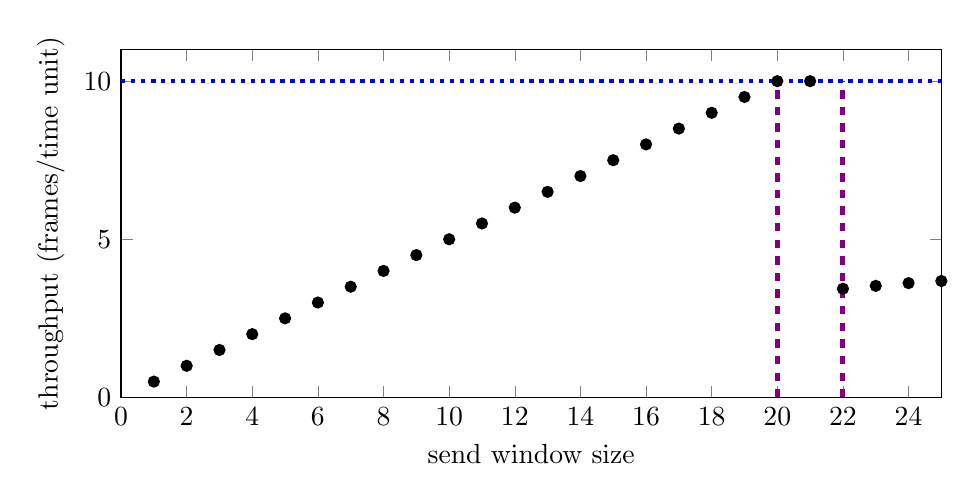
\begin{tikzpicture}
\begin{axis}[width=12cm,height=6cm,
    xlabel=send window size,
    ylabel=throughput (frames/time unit),
    xmin=0,xmax=25,ymin=0]
\addplot[only marks] coordinates {
(1, 0.5000025000125)
(2, 1.0000090000810007)
(3, 1.4999925000374998)
(4, 2.0000280003920055)
(5, 2.500037500562508)
(6, 3.000003000003)
(7, 3.5000035000035)
(8, 4.000048000576006)
(9, 4.499842505512307)
(10, 5.000025000125)
(11, 5.499975250111374)
(12, 5.99977200866367)
(13, 6.499710762871052)
(14, 6.999811005102861)
(15, 7.4996812635462975)
(16, 7.999680012799485)
(17, 8.499426288725509)
(18, 8.999361045365776)
(19, 9.499202067026369)
(20, 9.999100080971061)
(21, 9.999100080973866)
(22, 3.435635094325549)
(23, 3.5274986154570636)
(24, 3.613708966335035)
(25, 3.6808686850100703)
(26, 3.753260645186032)
(27, 3.8487443471573166)
(28, 3.925956461143474)
};
\addplot[blue,dotted,ultra thick,domain=0:25] {10};
    \draw[violet,dashed,ultra thick] (axis cs:20,0) -- (axis cs:20, 10)
     coordinate (empty queue mark);
    \draw[violet,dashed,ultra thick] (axis cs:21.99,0) -- (axis cs:21.99, 10)
     coordinate (full queue mark);
\end{axis}
\end{tikzpicture}
\end{frame}

\begin{frame}[fragile,label=transitTime]{packet transit time}
\begin{tikzpicture}
\draw[ultra thick,arrows={-Latex}] (0, 0) node[left] {sender} -- (1, 0);
\draw[thick] (1, -.5) rectangle (3, .5);
\foreach \x in {2,2.2,2.4,2.6,2.8} {
    \draw (\x, -.5) -- (\x, .5);
}
\node[anchor=south,align=center] at (2, .5) {
    loss when full
};
\node[anchor=north,align=center] at (2, -.5) (queue label) {
    queue
};
\node[anchor=north,font=\fontsize{9}{10}\selectfont] at ([yshift=.3cm]queue label.south) {
    capacity 20
};
\draw[ultra thick,arrows={-Latex}] (3, 0) -- (12, 0) node[right]{receiver}
    node[midway,fill=white,draw=black,very thick,align=left] {
        10 data frames/time unit \\
        1 time unit delay
    }
    node[visible on=<1-3>,ultra thick,pos=0,draw=black,fill=white,font=\tiny,below=.5cm] (data-main) {data};
    \begin{visibleenv}<2->
    \draw[red,-Latex,very thick] (data-main.east) -- (data-main.west -| 13, 0) coordinate (end send)
        node[midway,below,font=\small] {1 time unit (sender to receiver)};
    \end{visibleenv}
\begin{scope}[shift={(12, -4)},x=-1cm]
    \draw[ultra thick,arrows={-Latex}] (0, 0) node[right] {receiver} -- (1, 0);
    \draw[thick] (1, -.5) rectangle (3, .5);
    \foreach \x in {2,2.2,2.4,2.6,2.8} {
        \draw (\x, -.5) -- (\x, .5);
    }
    \node[anchor=south,align=center] at (2, .5) {
        loss when full
    };
    \node[anchor=north,align=center] at (2, -.5) (queue label) {
        queue
    };
    \node[anchor=north,font=\small] at ([yshift=.2cm]queue label.south) {
        capacity 20
    };
    \draw[ultra thick,arrows={-Latex}] (3, 0) -- (12, 0) node[left]{sender}
        node[midway,fill=white,draw=black,very thick,align=left] {
            100 ACK frames/time unit \\
            1 time unit delay
        }
        node[visible on=<2->,pos=0,draw=red,fill=white,font=\tiny,below=.5cm,align=center,inner sep=0.5mm] 
            (ack-start) {a\\c\\k};
    \begin{visibleenv}<2->
        \draw[dotted,red,-Latex,very thick] (end send) |- (ack-start.east);
        \draw[red,-Latex,very thick] (ack-start.west) -- (ack-start.west -| 12, 0) node[midway,below,font=\small] { + 1 time unit (receiver to sender)};
    \end{visibleenv}
\end{scope}
\begin{visibleenv}<3>
\node[draw=red,fill=white,ultra thick,align=left] at (6, -2.5) {
    takes 1 + 1 time units to send message + receive ack \\
    goal: keep sending stuff while waiting
};
\end{visibleenv}
\end{tikzpicture}
\end{frame}

\begin{frame}{filling the pipe}
    \begin{itemize}
    \item round-trip time of 2 time units
        \begin{itemize}
        \item from send data to receive ACK (assuming no queuing delay)
        \end{itemize}
    \item can send 10 data frames per time unit
    \item = can send 20 data frames while waiting for ACK
    \vspace{.5cm}
    \item<2> \myemph{``bandwidth-delay product''}
        \begin{itemize}
        \item 10/time unit (banwidth) times 2 time unit (RTT = delay)
        \end{itemize}
    \end{itemize}
\end{frame}

\begin{frame}[fragile,label=throughAndWindow]{throughput and window size (detail)}
\begin{tikzpicture}
\begin{axis}[width=12cm,height=6cm,
    xlabel=send window size,
    ylabel=throughput (frames/time unit),
    xmin=17,xmax=24,ymin=0]
\addplot[only marks] coordinates {
(1, 0.5000025000125)
(2, 1.0000090000810007)
(3, 1.4999925000374998)
(4, 2.0000280003920055)
(5, 2.500037500562508)
(6, 3.000003000003)
(7, 3.5000035000035)
(8, 4.000048000576006)
(9, 4.499842505512307)
(10, 5.000025000125)
(11, 5.499975250111374)
(12, 5.99977200866367)
(13, 6.499710762871052)
(14, 6.999811005102861)
(15, 7.4996812635462975)
(16, 7.999680012799485)
(17, 8.499426288725509)
(18, 8.999361045365776)
(19, 9.499202067026369)
(20, 9.999100080971061)
(21, 9.999100080973866)
(22, 3.435635094325549)
(23, 3.5274986154570636)
(24, 3.613708966335035)
(25, 3.6808686850100703)
(26, 3.753260645186032)
(27, 3.8487443471573166)
(28, 3.925956461143474)
};
\addplot[blue,dotted,ultra thick,domain=0:25] {10};
    \draw[violet,dashed,ultra thick] (axis cs:20,0) -- (axis cs:20, 11)
     coordinate (empty queue mark);
    \draw[violet,dashed,ultra thick] (axis cs:21.99,0) -- (axis cs:21.99, 11)
     coordinate (full queue mark);
\end{axis}
\node[violet,anchor=south east,align=right] (nq) at ([xshift=1.5cm]empty queue mark) {
    (no queuing delay)
};
\node[violet,anchor=south west,align=left] (mq) at ([xshift=-1.5cm]full queue mark) {
    (max queuing delay)
};
\node[violet,anchor=south] at ($(nq)!0.5!(mq)$) {bandwidth-delay product};
\end{tikzpicture}
\end{frame}


\begin{frame}[fragile,label=fullPipe]{filling the pipe}
\begin{tikzpicture}
\draw[ultra thick,arrows={-Latex}] (0, 0) node[left] {sender} -- (1, 0);
\draw[thick] (1, -.5) rectangle (3, .5);
\foreach \x in {2,2.2,2.4,2.6,2.8} {
    \draw (\x, -.5) -- (\x, .5);
}
\node[anchor=south,align=center] at (2, .5) {
    loss when full
};
\node[anchor=north,align=center] at (2, -.5) (queue label) {
    queue
};
\node[anchor=north,font=\fontsize{9}{10}\selectfont] at ([yshift=.3cm]queue label.south) {
    capacity 20
};
\draw[ultra thick,arrows={-Latex}] (3, 0) -- (12, 0) node[right]{receiver}
    node[midway,fill=white,draw=black,very thick,align=left] {
        10 data frames/time unit \\
        1 time unit delay
    }
    \foreach \x in {0,1,2,3,4,5,6,7,8,9} {
        node[visible on=<3->,pos=\x*.1+0.05,draw=black,fill=white,font=\tiny,below=.5cm] (data-\x) {data}
    };
    \begin{visibleenv}<3->
    \draw[red,Latex-Latex] ([yshift=-.1cm]data-0.south west) -- ([yshift=-.1cm]data-1.south west)
        node[below,font=\small] {0.1 time unit};
    \end{visibleenv}
\begin{scope}[shift={(12, -4)},x=-1cm]
    \draw[ultra thick,arrows={-Latex}] (0, 0) node[right] {receiver} -- (1, 0);
    \draw[thick] (1, -.5) rectangle (3, .5);
    \foreach \x in {2,2.2,2.4,2.6,2.8} {
        \draw (\x, -.5) -- (\x, .5);
    }
    \node[anchor=south,align=center] at (2, .5) {
        loss when full
    };
    \node[anchor=north,align=center] at (2, -.5) (queue label) {
        queue
    };
    \node[anchor=north,font=\small] at ([yshift=.2cm]queue label.south) {
        capacity 20
    };
    \draw[ultra thick,arrows={-Latex}] (3, 0) -- (12, 0) node[left]{sender}
        node[midway,fill=white,draw=black,very thick,align=left] {
            100 ACK frames/time unit \\
            1 time unit delay
        }
        \foreach \x in {0,1,2,3,4,5,6,7,8,9} {
            node[visible on=<3->,pos=\x*.1+0.05,draw=black,fill=white,font=\tiny,below=.5cm,align=center,inner sep=0.5mm] {a\\c\\k}
        };
\end{scope}
\end{tikzpicture}
\end{frame}


\subsection{problems solved}
\begin{frame}{sliding windows solve\ldots}
    \begin{itemize}
    \item reliability on unrelaible link
    \item \textit{congestion control}
        \begin{itemize}
        \item keep network from being overloaded
        \item \ldots by having window sizes set correctly
        \end{itemize}
    \item \textit{flow control}
        \begin{itemize}
        \item keep sender from getting too far ahead of sender
        \item \ldots by having window sizes set correctly
        \end{itemize}
    \end{itemize}
\end{frame}


\subsection{sequence number wraparound}
\usetikzlibrary{arrows.meta, calc, fit, matrix, patterns, shapes.misc}

\providecommand{\computer}{%
    
\includegraphics[width=1cm]{../common/Noun_project_216.pdf}
}
\providecommand{\switch}{%
    
\includegraphics[width=0.9cm]{../common/fig-switch.pdf}
}
\providecommand{\bigswitch}{%
    
\includegraphics[width=1.4cm]{../common/fig-switch.pdf}
}
\providecommand{\router}{%
    
\includegraphics[width=0.9cm]{../common/fig-router.pdf}
}


\begin{frame}{sequence number wraparound}
    \begin{itemize}
    \item protocol so far requires arbitrarily large sequence numbers
        \begin{itemize}
        \item doing $<$ and $>$ checks on sequence number, so they need to increase
        \end{itemize}
    \item would like to use smaller sequence numbers
        \begin{itemize}
        \item think: transferring multi-gigabyte file
        \end{itemize}
    \item question: what goes wrong when we reuse sequeunce numbers?
    \end{itemize}
\end{frame}

\begin{frame}{sender/receiver desync: missing ACKs}
\begin{tikzpicture}
\tikzset{
    seqlist/.style={tight matrix,nodes={text width=.8cm,minimum height=.8cm},column sep=.6mm},
    dots/.style={draw=none,execute at begin node=\ldots,anchor=center,font=\huge,text width=1cm,align=center},
    region mark/.style={very thick,decorate,decoration={brace,mirror}},
    region mark label/.style={midway,below,align=center},
    verified/.style={pattern color=black!30,pattern=checkerboard},
    ack sent not recvd/.style={fill=blue!60},
    unsent ready/.style={pattern color=yellow!30!black,pattern=checkerboard},
    unsent/.style={pattern=crosshatch dots,pattern color=violet!70},
}
\begin{scope}[name prefix=s-]
    \matrix[seqlist] (window) {
        |[dots,alias=window-start]| ~ \& |[alias=after-window-start,verified,alias=LAR]| ~ \&
        |[ack sent not recvd,alias=after LAR]| ~ \& |[ack sent not recvd]| ~ \& |[ack sent not recvd]| ~ \& 
        |[ack sent not recvd,alias=LFS]| ~ \& 
        |[alias=after LFS,unsent]| ~ \& |[unsent,alias=before-window-end]| ~  \&
        |[unsent]| ~  \&
        |[unsent]| ~  \&
        |[unsent]| ~  \&
        |[unsent,alias=before-window-end]| ~  \&
        \& |[alias=window-end,dots]| \\
    };
    \node[anchor=east] at (window-start.west) {sender};
    \draw[thick,Latex-] (LAR.north) -- ++(0,.5) node[above,align=center] (LAR label) {(LAR)\\last ACK recv'd};
    \draw[thick,Latex-] (LFS.north) -- ++(0,.5) node[above,align=center] (LFS label) {(LFS)\\last frame sent};
\end{scope}
\begin{scope}[name prefix=r-,yshift=-3cm]
    \matrix[seqlist] (window) {
        |[dots,alias=window-start]| ~ \& |[alias=after-window-start,verified]| ~ \& 
        |[alias=after LAR,ack sent not recvd]| ~ \& |[ack sent not recvd]| ~ \& 
        |[ack sent not recvd]| ~ \& |[alias=LFR,ack sent not recvd]| ~ \&
        |[unsent ready,alias=after LFR]| ~ \& |[unsent ready,alias=after after LFR]| ~ \&
        |[unsent ready]| ~ \& |[unsent ready,alias=LAF]| ~ \& 
        |[alias=after LAF,unsent]| ~ \& |[unsent,alias=before-window-end]| ~ \& |[alias=window-end,dots]| \\
    };
    \node[anchor=east] at (window-start.west) {receiver};
    \draw[thick,Latex-] (LFR.north) -- ++(0,.5) node[above,align=center] {(LFR)\\last frame recv'd*};
    \draw[thick,Latex-] (LAF.north) -- ++(0,.5) node[above,align=center] {(LAF)\\last accepted frame};
    \draw[region mark] ([yshift=-.1cm]after LAR.south west) -- ([yshift=-.1cm]LFR.south east)
        node[region mark label] {resent if \\ ACK lost};
    \draw[region mark] ([yshift=-.1cm]after LFR.south west) -- ([yshift=-.1cm]LAF.south east)
        node[region mark label] {expected if \\ ACK not lost};
\end{scope}
\begin{visibleenv}<2->
\node[draw=red,ultra thick,fit=(s-after LAR) (r-LAF),label={[red,align=left,fill=white,fill opacity=0.95]west:need unique \\ numbers for all these}] {};
\end{visibleenv}
\begin{visibleenv}<3->
\foreach \x/\lbl in {2/4,3/5,4/6,5/7,6/0,7/1,8/2,9/3,10/4,11/5,12/6,13/7} {
    \node[fill=white,font=\small,text=red,circle,draw=red,ultra thick,anchor=south west,inner sep=0.1mm] at ([xshift=\x * .935cm - 0.4cm]s-window-start.north west) {\lbl};
}
\end{visibleenv}
\end{tikzpicture}
\end{frame}

\begin{frame}{wraparound}
\begin{tikzpicture}
\tikzset{
    box/.style={thick},
    message/.style={draw,thick,-Latex},
    failure/.style={draw,ultra thick,red,cross out,minimum width=1cm,minimum height=1cm},
    every node/.style={inner sep=0.1mm},
}
\begin{scope}[xshift=1cm,x=0.9cm,y=0.9cm]
\draw[box] (0, 0) rectangle ++(2, -8) 
    node[midway,align=center] {machine\\A};
\draw[box] (13, 0) rectangle ++(2, -8) 
    node[midway,align=center] {machine\\B};
\draw[message] (2, -0.5) -- (13, -1.5) node[pos=0.25,above,sloped] {\myemph{0}: ``The ''};
\draw[message] (13, -1.75) -- (2, -2.75) node[pos=0.25,sloped,below] {got up to \myemph{0}};
\draw[message] (2, -1) -- (13, -2) node[pos=0.25, above, sloped] {\myemph{1}: ``meeting''};
\draw[message] (13, -2.25) -- (2, -3.25) node[pos=0.25, sloped,below] {got up to \myemph{1}};

% in response to got 0
\draw[message] (2, -3) -- (13, -4) node[pos=0.5, above, sloped] {\myemph{2}: ``is''};
\draw[message] (13, -4.25) -- (2, -5.25) node[pos=0.25, sloped,below] {got up to \myemph{2}};
% in response to got 1
\draw[message] (2, -3.5) -- (13, -4.5) node[pos=0.5, above, sloped] {\myemph{3}: ``at''};
\draw[message] (13, -4.75) -- (2, -5.75) node[pos=0.25, sloped,below] {got up to \myemph{3}};

% in response to got 2
\draw[message] (2, -5.5) -- (13, -6.5) node[pos=0.5, above, sloped] {\myemph{0}: ``12pm''};
\draw[message] (13, -6.75) -- (2, -7.75) node[pos=0.25, sloped,below] {got up to \myemph{0}};
\end{scope}
\end{tikzpicture}
\end{frame}

\begin{frame}{loss and resend?}
\begin{tikzpicture}
\tikzset{
    box/.style={thick},
    message/.style={draw,thick,-Latex,font=\small},
    failure/.style={draw,ultra thick,red,cross out,minimum width=1cm,minimum height=1cm},
    every node/.style={inner sep=0.1mm},
}
\begin{scope}[xshift=1cm,x=0.9cm,y=0.7cm]
\draw[box] (0, 2) rectangle ++(2, -10) 
    node[midway,align=center] {machine\\A};
\draw[box] (13, 2) rectangle ++(2, -10) 
    node[midway,align=center] {machine\\B};
\draw[message] (2, 2-0.5) -- (9, 2-1.2) node[pos=0.25,above,sloped] {\myemph{0}: ``The ''} node[failure] {};
\draw[message] (2, 2-1) -- (9, 2-1.8) node[pos=0.25, above, sloped] {\myemph{1}: ``meeting''} node[failure] {};
\draw[message] (13, -2.25) -- (2, -3.25) node[pos=0.25, sloped,below] {got up to \myemph{1}};
\draw[message] (2, -0.5) -- (13, -1.5) node[pos=0.25,above,sloped] {\myemph{0}: ``The ''};
\draw[message] (13, -1.75) -- (2, -2.75) node[pos=0.25,sloped,below] {got up to \myemph{0}};
\draw[message] (2, -1) -- (13, -2) node[pos=0.25, above, sloped] {\myemph{1}: ``meeting''};
\draw[message] (13, -2.25) -- (2, -3.25) node[pos=0.25, sloped,below] {got up to \myemph{1}};

% in response to got 0
\draw[message] (2, -3) -- (13, -4) node[pos=0.5, above, sloped] {\myemph{2}: ``is''};
\draw[message] (13, -4.25) -- (2, -5.25) node[pos=0.25, sloped,below] {got up to \myemph{2}};
% in response to got 1
\draw[message] (2, -3.5) -- (13, -4.5) node[pos=0.5, above, sloped] {\myemph{3}: ``at''};
\draw[message] (13, -4.75) -- (2, -5.75) node[pos=0.25, sloped,below] {got up to \myemph{3}};

% in response to got 2
\draw[message] (2, -5.5) -- (13, -6.5) node[pos=0.5, above, sloped] {\myemph{0}: ``12pm''};
\draw[message] (13, -6.75) -- (2, -7.75) node[pos=0.25, sloped,below] {got up to \myemph{0}};
\end{scope}
\end{tikzpicture}
\end{frame}

\begin{frame}{very bad reordering}
\begin{tikzpicture}
\tikzset{
    box/.style={thick},
    message/.style={draw,thick,-Latex,font=\small},
    failure/.style={draw,ultra thick,red,cross out,minimum width=1cm,minimum height=1cm},
    every node/.style={inner sep=0.1mm},
}
\begin{scope}[xshift=1cm,x=0.9cm,y=0.7cm]
\draw[box] (0, 2) rectangle ++(2, -10) 
    node[midway,align=center] {machine\\A};
\draw[box] (13, 2) rectangle ++(2, -10) 
    node[midway,align=center] {machine\\B};
\draw[message] (2, 2-0.5) -- (13, -6) node[pos=0.1,above,sloped,font=\bfseries] {\myemph{0}: ``The ''};
\draw[message] (2, 2-1) -- (9, 2-1.8) node[pos=0.75, above, sloped] {\myemph{1}: ``meeting''} node[failure] {};
\draw[message] (13, -2.25) -- (2, -3.25) node[pos=0.25, sloped,below] {got up to \myemph{1}};
\draw[message] (2, -0.5) -- (13, -1.5) node[pos=0.25,above,sloped] {\myemph{0}: ``The ''};
\draw[message] (13, -1.75) -- (2, -2.75) node[pos=0.25,sloped,below] {got up to \myemph{0}};
\draw[message] (2, -1) -- (13, -2) node[pos=0.25, above, sloped] {\myemph{1}: ``meeting''};
\draw[message] (13, -2.25) -- (2, -3.25) node[pos=0.25, sloped,below] {got up to \myemph{1}};

% in response to got 0
\draw[message] (2, -3) -- (13, -4) node[pos=0.5, above, sloped] {\myemph{2}: ``is''};
\draw[message] (13, -4.25) -- (2, -5.25) node[pos=0.25, sloped,below] {got up to \myemph{2}};
% in response to got 1
\draw[message] (2, -3.5) -- (13, -4.5) node[pos=0.5, above, sloped] {\myemph{3}: ``at''};
\draw[message] (13, -4.75) -- (2, -5.75) node[pos=0.25, sloped,below] {got up to \myemph{3}};

% in response to got 2
\draw[message] (2, -5.5) -- (13, -6.5) node[pos=0.5, above, sloped,font=\bfseries] {\myemph{0}: ``12pm''};
% in response to BOGUS got 0
\draw[message] (13, -6.25) -- (2, -7.25) node[pos=0.25, sloped,below] {got up to \myemph{0}};
\end{scope}
\end{tikzpicture}
\end{frame}

\begin{frame}{possible reason}
\begin{tikzpicture}
\tikzset{
    connect one/.style={draw,very thick,Latex-Latex},
    computer/.style={inner sep=0mm,outer sep=0mm,execute at begin node={\computer}},
    switch/.style={inner sep=0mm,outer sep=0mm,execute at begin node={\switch}},
    router/.style={inner sep=0mm,outer sep=0mm,execute at begin node={\router}},
    big switch/.style={inner sep=0mm,outer sep=0mm,execute at begin node={\bigswitch}},
    packet/.style={minimum width=.4cm,minimum height=0.2cm,inner sep=0mm,outer sep=0mm,draw},
    packet lg/.style={minimum width=.6cm,minimum height=0.2cm,inner sep=0mm,outer sep=0mm,draw},
}
\node[computer] (start) at (0,0) {};
\node[computer] (end)  at (13,0) {};
\node[router] (pre1) at (3, 3) {};
\node[router] (pre2) at (4, .5) {};
\node[router] (pre3) at (5, 3) {};
\node[router] (A) at (6, 1) {};
\node[router] (B) at (7, -1) {};
\node[router] (C) at (8, 3) {};
\node[router] (D) at (11, 0) {};
\
\node[router] (E) at (7.5, -2) {};
\foreach \x/\y in {start/pre1,pre1/pre2,pre2/pre3,pre3/A,A/B,B/C,C/D,D/end,start/E,E/end} {
    \draw[connect one] (\x) -- (\y);
}
\node[font=\small,draw,fill=white] at ($(C)!0.5!(D)$) {\myemph{0}: ``The ''};
\node[font=\small,draw,fill=white] at ($(E)!0.7!(start)$) {\myemph{0}: ``12pm''};
\end{tikzpicture}
\end{frame}


\section{TCP example}

\subsection{TCP segment format}
\usetikzlibrary{patterns}
\begin{frame}{TCP}
    \begin{itemize}
    \item transmission control protocol (TCP)
    \item implements reliable streams of bytes
    \item similar mechanism to what we've described
    \end{itemize}
\end{frame}

\begin{frame}{TCP extras/differences}
    \begin{itemize}
    \item bidirectional ---
        \begin{itemize}
        \item separate sequence numbers in each direction
        \item can combine data (from A to B) with acknowledgment (from B to A)
        \end{itemize}
    \item sequence numbers are byte numbers ---
        \begin{itemize}
        \item can retransmit data in different sized packets
        \item sequence numbers = index of \textit{first byte} sent
        \item acknowledgment numbers = index of \textit{last byte} acknowledged
        \end{itemize}
    \item dynamic/variable window sizes
        \begin{itemize}
        \item we'll discuss strategies later
        \end{itemize}
    \item offical name for packets = \textit{segments}
    \end{itemize}
\end{frame}

\begin{frame}[fragile]{TCP segment format}
\begin{tikzpicture}
    \tikzset{
        box/.style={draw,thick},
        box unused/.style={draw,thick,pattern=north west lines},
        box label/.style={midway,font=\small,align=center},
        box label flags/.style={midway,font=\fontsize{8}{9}\selectfont,align=center},
        hi on/.style={alt=<#1>{ultra thick,fill=red!10}},
        explain box 1/.style={draw=red,line width=0.8mm,fill=white,anchor=center,at={(explain box loc 1)},align=center},
        explain box 2/.style={draw=red,line width=0.8mm,fill=white,anchor=center,at={(explain box loc 2)},align=center},
        explain box 3/.style={draw=red,line width=0.8mm,fill=white,anchor=center,at={(explain box loc 3)},align=center},
    }
    \begin{scope}[x=4.7mm,y=9mm]
        \coordinate (explain box loc 1) at (16, -3.1);
        \coordinate (explain box loc 2) at (16, -5.1);
        \coordinate (explain box loc 3) at (16, -1.1);
        \path[shading=axis,top color=white,bottom color=black!20] (0, 1) rectangle (32, 0)
            node[box label] {(lower layer header)};
        \path[box,hi on=2] (0, 0) rectangle (16, -1) node[box label] {source port (16b)};
        \path[box,hi on=2] (16, 0) rectangle (32, -1) node[box label] {destination port (16b)};
        \path[box,hi on=3] (0, -1) rectangle (32, -2) node[box label] {sequence number (32b)};
        \path[box,hi on=4] (0, -2) rectangle (32, -3) node[box label] {acknowledgment number (32b)};
        \path[box,hi on=10] (0, -3) rectangle (4, -4) node[box label] {data offset\\(4b)};
        \path[box unused] (4, -3) rectangle (8, -4);
        \path[box,hi on=9] (8, -3) rectangle ++(1, -1) node[box label flags]{C\\W\\R};
        \path[box,hi on=9] (9, -3) rectangle ++(1, -1) node[box label flags]{E\\C\\E};
        \path[box,hi on=6] (10, -3) rectangle ++(1, -1) node[box label flags]{U\\R\\G};
        \path[box,hi on=4] (11, -3) rectangle ++(1, -1) node[box label flags]{A\\C\\K};
        \path[box,hi on=7] (12, -3) rectangle ++(1, -1) node[box label flags]{P\\S\\H};
        \path[box,hi on=8] (13, -3) rectangle ++(1, -1) node[box label flags]{R\\S\\T};
        \path[box,hi on=8] (14, -3) rectangle ++(1, -1) node[box label flags]{S\\Y\\N};
        \path[box,hi on=8] (15, -3) rectangle ++(1, -1) node[box label flags]{F\\I\\N};
        \path[box,hi on=5] (16, -3) rectangle ++(16, -1) node[box label] {window size (16b)};
        \path[box] (0, -4) rectangle ++(16, -1) node[box label] {checksum (16b)};
        \path[box, hi on=6] (16, -4) rectangle ++(16, -1) node[box label] {urgent pointer (16b)};
        \path[box,hi on=10] (0, -5) rectangle ++(32, -1) node[box label] {options (variable)};
        \draw[line width=1mm,white] (-.2, -5.55) -- (.2, -5.45);
        \draw[line width=1mm,white] (32 -.2, -5.55) -- (32 + .2, -5.45);
        \draw[very thick,black] (-.2, -5.5) -- (.2, -5.4);
        \draw[very thick,black] (32 -.2, -5.5) -- (32 + .2, -5.4);
        \draw[very thick,black] (-.2, -5.6) -- (.2, -5.5);
        \draw[very thick,black] (32 -.2, -5.6) -- (32 + .2, -5.5);
        \path[overlay,shading=axis,top color=black!20,bottom color=white] (0, -6) rectangle (32, -7)
            node[box label] {(data)};
    \end{scope}
    \begin{visibleenv}<2>
        \node[explain box 1] {
            ports identify program/socket on machines \\
            (we'll talk more when we cover sockets) \\
            ~ \\
            machines identified in lower layer headers 
        };
    \end{visibleenv}
    \begin{visibleenv}<3>
        \node[explain box 2] {
            byte number for first byte of data in this packet
        };
    \end{visibleenv}
    \begin{visibleenv}<4>
        \node[explain box 2] {
            ack number = byte number of largest byte acknowledged \\
            only meaningful if ACK `flag' is 1
        };
    \end{visibleenv}
    \begin{visibleenv}<5>
        \node[explain box 3] {
            window size is receive window size \\
            tells sender how much receiver will accept \\
            sender window could/often will be different \\
            (and not directly visible in packets)
        };
    \end{visibleenv}
    \begin{visibleenv}<6>
        \node[explain box 3] {
            some fields related to `urgent data' mechanism \\
            almost never used today
        };
    \end{visibleenv}
    \begin{visibleenv}<7>
        \node[explain box 3] {
            PSH (push) `flag' is hint that sender does not have \\
            more data to send right away
        };
    \end{visibleenv}
    \begin{visibleenv}<8>
        \node[explain box 3] {
            RST (reset), SYN (synchornize), FIN flags \\
            used for connnection management \\
            (we'll talk more when we cover sockets)
        };
    \end{visibleenv}
    \begin{visibleenv}<9>
        \node[explain box 3] {
            CWR (congestion window reduced) and \\
            ECE (explicit congestion notification echo) flags \\
            sometimes used as part of setting window size \\
            to match network conditions (later topic for us)
        };
    \end{visibleenv}
    \begin{visibleenv}<10>
        \node[explain box 3] {
            header can have variable number of ``options'' \\
            technically optional, almost always used today \\
            ~ \\
            size of header indicated by \textit{data offset} \\
            (data offset is units of 32-bit words, not bytes)
        };
    \end{visibleenv}
\end{tikzpicture}
\end{frame}

\begin{frame}{exercise: maximum throughput}
    \begin{itemize}
    \item let's say we have a receiver window size of 65535 bytes
    \item and a round-trip time of 100 ms
    \vspace{.5cm}
    \item if we want to avoid sending data the sender will reject as outside
    its window, maximum throughput?
    \end{itemize}
\begin{tabular}{ll}
A. around 32kbyte/sec &
B. around 64kbyte/sec \\
C. around 128kbyte/sec &
D. around 320kbyte/sec \\
E. around 640kbyte/sec &
F. around 1280kbyte/sec \\
G. something else \\
\end{tabular}
\end{frame}

\begin{frame}{selected TCP options}
    \begin{itemize}
    \item window size scale factor
        \begin{itemize}
        \item allow receiver window sizes greater than 64k
        \item needed to get reasonable bandwidth on modern networks
        \end{itemize}
    \item timestamps
        \begin{itemize}
        \item allow figuring out round trip time to estimate timeout
        \item extend 32-bit sequence number, which is too small for multi-gigabit networks
        \end{itemize}
    \item selective acknowledgements
        \begin{itemize}
        \item allow providing information about `holes' in received data
        \item example: I got bytes 1--5000, 6000--7000, 8000--9000
        \item without it would only say 5000
        \end{itemize}
    \end{itemize}
\end{frame}

\begin{frame}[fragile]{selected TCP option formats}
\begin{tikzpicture}
    \tikzset{
        box/.style={draw,thick},
        box unused/.style={draw,thick,pattern=north west lines},
        box label/.style={midway,font=\small,align=center},
        box label flags/.style={midway,font=\fontsize{8}{9}\selectfont,align=center},
        hi on/.style={alt=<#1>{ultra thick,fill=red!10}},
        explain box 1/.style={draw=red,line width=0.8mm,fill=white,anchor=center,at={(explain box loc 1)},align=center},
        explain box 2/.style={draw=red,line width=0.8mm,fill=white,anchor=center,at={(explain box loc 2)},align=center},
        explain box 3/.style={draw=red,line width=0.8mm,fill=white,anchor=center,at={(explain box loc 3)},align=center},
    }
    \begin{scope}[x=4.7mm,y=9mm]
        \coordinate (explain box loc 1) at (16, -5.1);
        \coordinate (explain box loc 2) at (16, -6.1);
        \coordinate (explain box loc 3) at (16, -1.1);
        \path[box,hi on=3] (0, 0) rectangle (8, -1) node[box label] {kind (8b)};
        \path[box,hi on=2] (8, 0) rectangle (16, -1) node[box label] {length (8b)};
        \path[shading=axis,left color=black!20,right color=white] (16, 0) rectangle (32, -1) node[box label] {option data};

        \node[anchor=south] at (16, -2) {\myemph<4>{window scale option}:};
        \path[box,hi on=4,hi on=3] (0, -2) rectangle ++(8, -1) node[box label] {\tt 3};
        \path[box,hi on=2,hi on=4] (8, -2) rectangle ++(8, -1) node[box label] {\tt 3};
        \path[box,hi on=4] (16, -2) rectangle ++(8, -1) node[box label] {shift count};
        
        \node[anchor=south] at (16, -4) {\myemph<5>{timestamps}:};
        \path[box,hi on=3] (0, -4) rectangle ++(8, -1) node[box label] {\tt 8};
        \path[box,hi on=2] (8, -4) rectangle ++(8, -1) node[box label] {\tt 10};
        \path[box] (16, -4) rectangle ++(16, -1) node[box label] {sender TS};
        \path[box,hi on=6] (0, -5) rectangle ++(16, -1) node[box label] {echoed TS};
    \end{scope}
    \begin{visibleenv}<2>
        \node[explain box 2] {
            length field permits skipping unrecognized options
        };
    \end{visibleenv}
    \begin{visibleenv}<3>
        \node[explain box 2] {
            unique kind codes for each option \\
            list of valid codes maintained by IANA \\
            (Internet Assigned Numbers Authority) 
        };
    \end{visibleenv}
    \begin{visibleenv}<4>
        \node[explain box 1] {
            sent only in connection setup \\
            only takes effect if both sides send it \\
            sets amount to left-shift \\
            all window size fields by
        };
    \end{visibleenv}
    \begin{visibleenv}<6>
        \node[explain box 3] {
            echoed timestamp --- \\
            only valid in ACK messages \\
            copy of timestamp sent in message ACK'd \\
            allows computing round-trip-time
        };
    \end{visibleenv}
\end{tikzpicture}
\end{frame}



%\subsection{TCP connection example 1}
%\begin{frame}{a TCP connection}
\begin{tikzpicture}
\tikzset{
    overlay box/.style={fill=white,fill opacity=0.9},
}
\node[overlay,anchor=north west,inner sep=0mm] (base) at (0, 0) {%
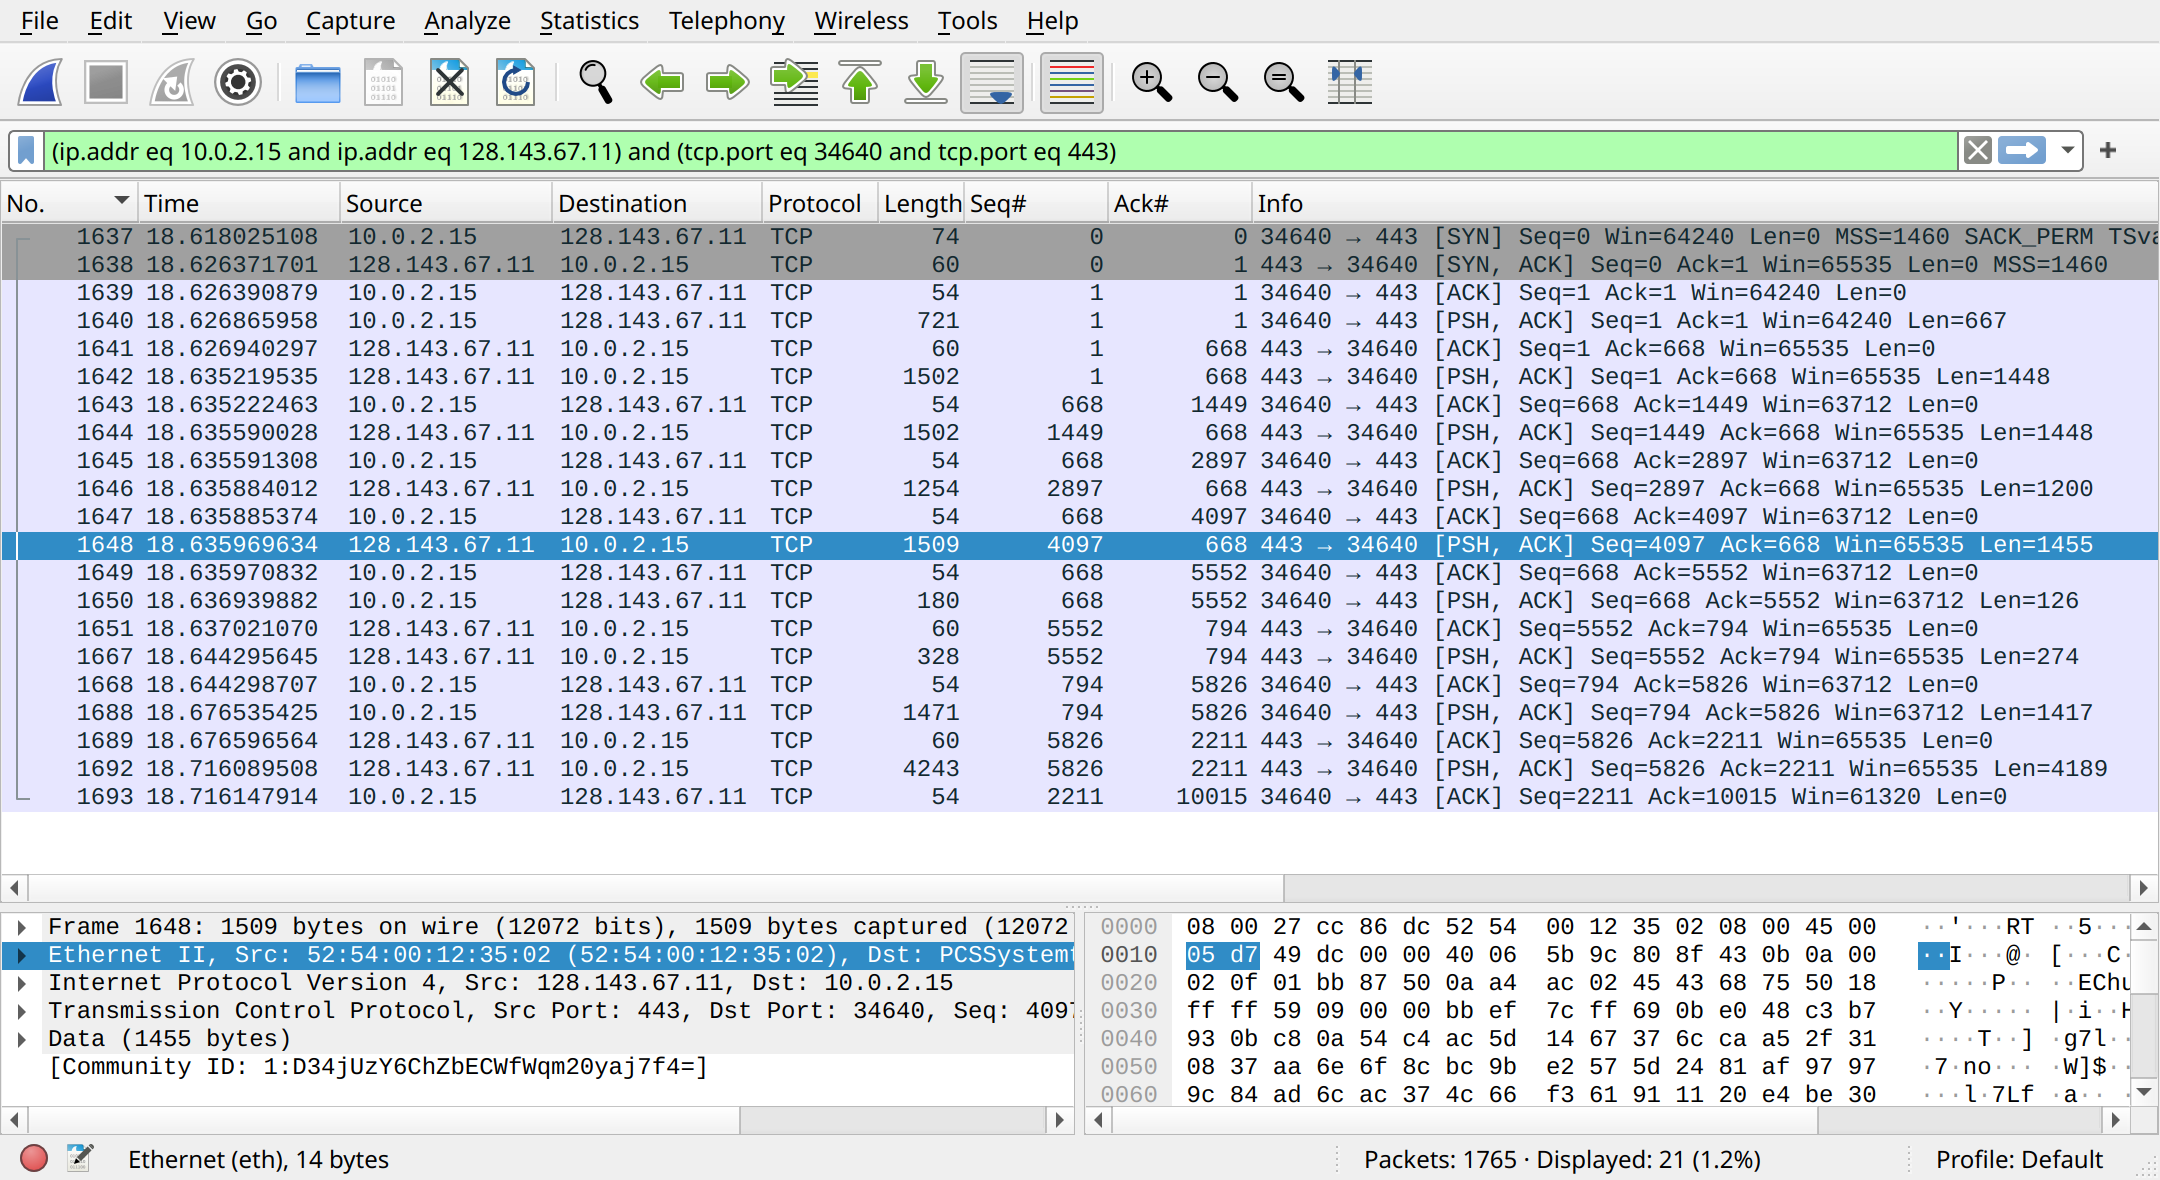
\includegraphics[width=\textwidth]{../reliable/wireshark-tcp-ex1-over}%
};
\path (0, 0) rectangle (14.5, -7); % for bounding box
\draw[overlay,help lines] (0, 0) grid (14, -8);
\begin{visibleenv}<2>

\end{visibleenv}
\end{tikzpicture}
\end{frame}


\subsection{TCP connection example}
\usetikzlibrary{shapes.geometric,spy}
\begin{frame}[fragile]{a TCP connection}
\tikzset{
    overlay box/.style={fill=white,fill opacity=0.95},
}
\begin{tikzpicture}[
    spy using outlines={%
        overlay,circle,magnification=2,size=2cm,connect spies,%
        every spy on node/.append style={very thick},%
        ultra thick,%
    }
]
\node[overlay,anchor=north west,inner sep=0mm] (base) at (0, 0) {%
\only<1-2>{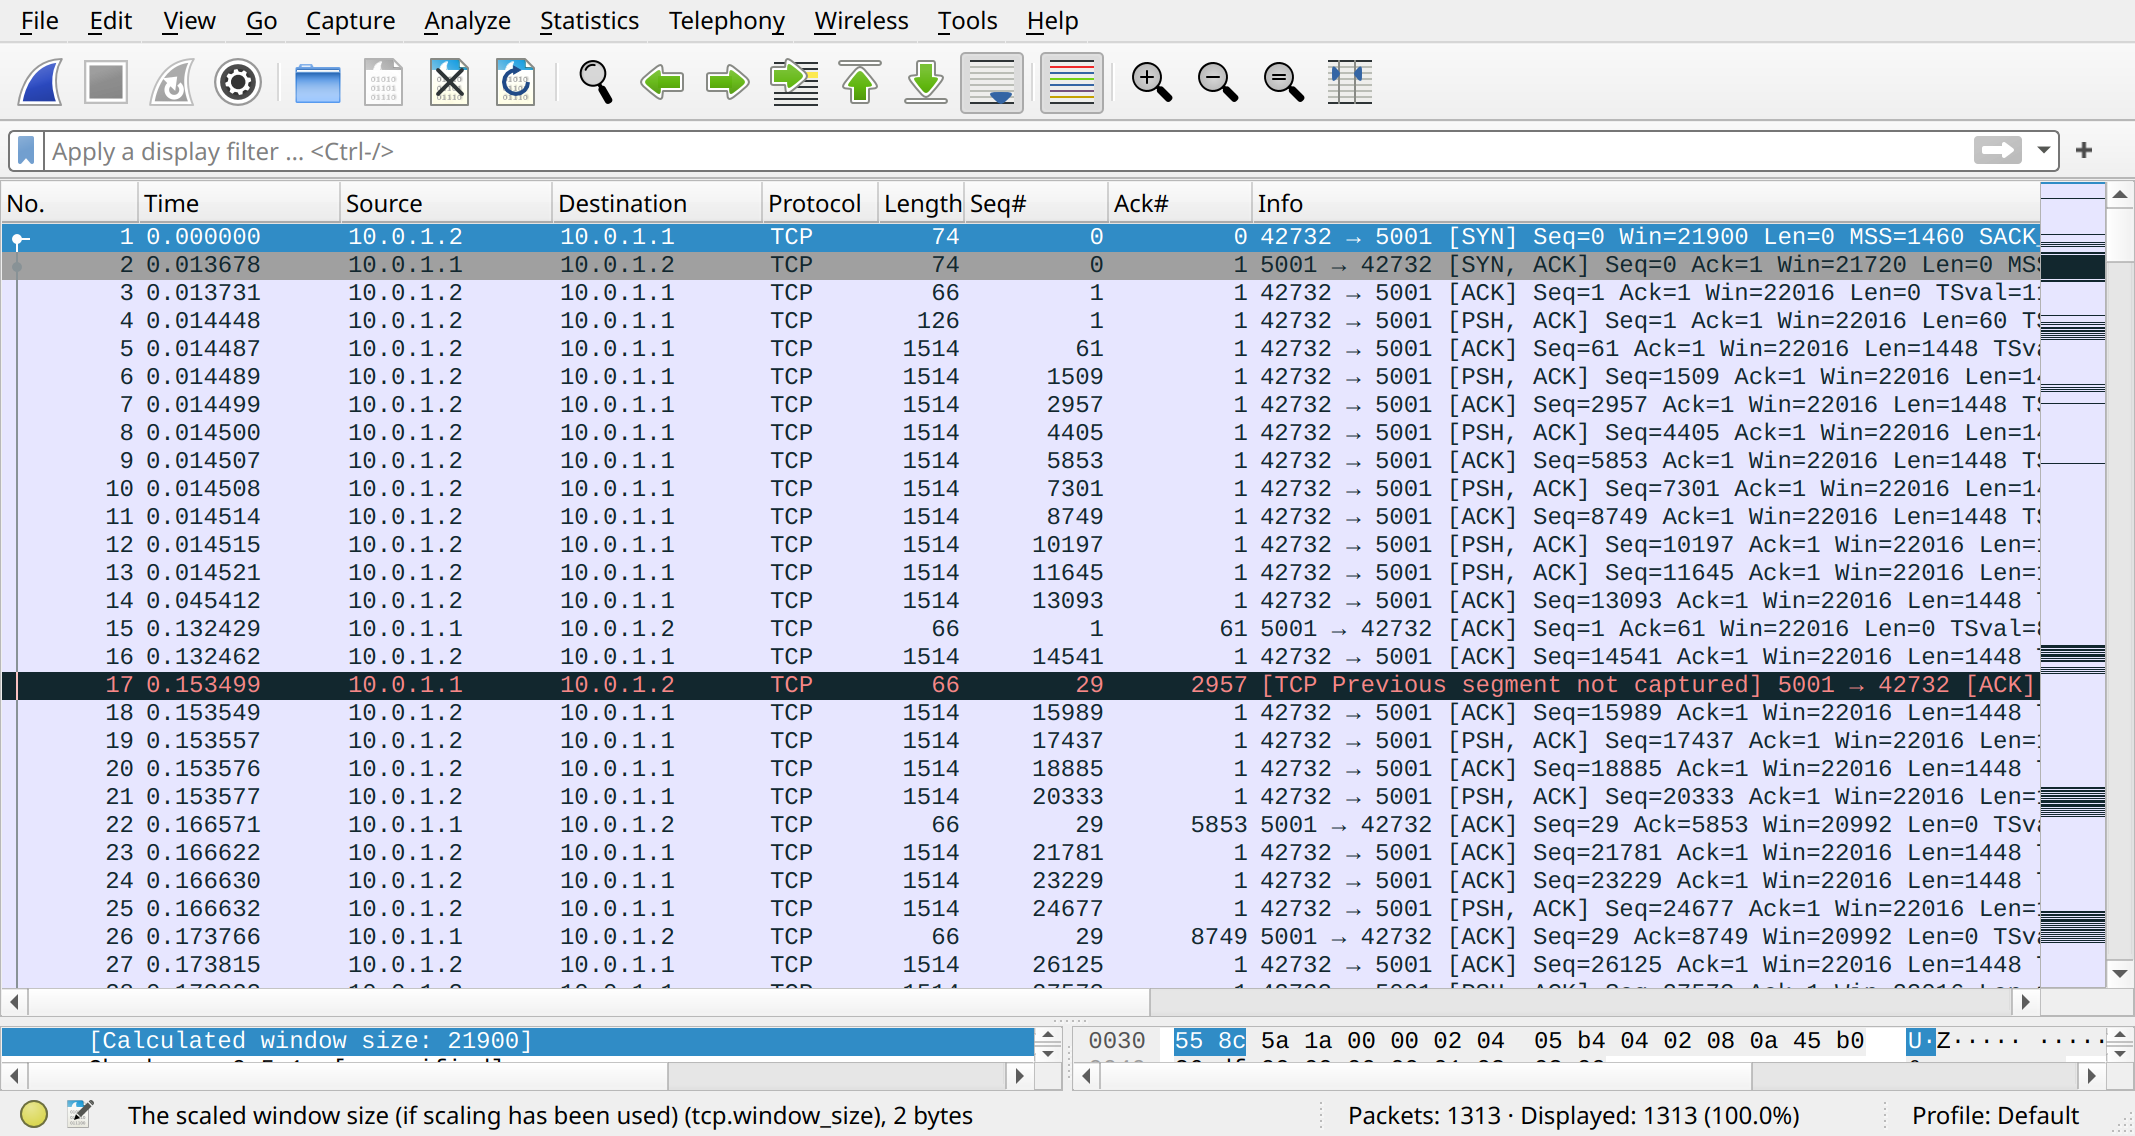
\includegraphics[width=\textwidth]{../reliable/wireshark-tcp-ex2-over}}%
\only<3->{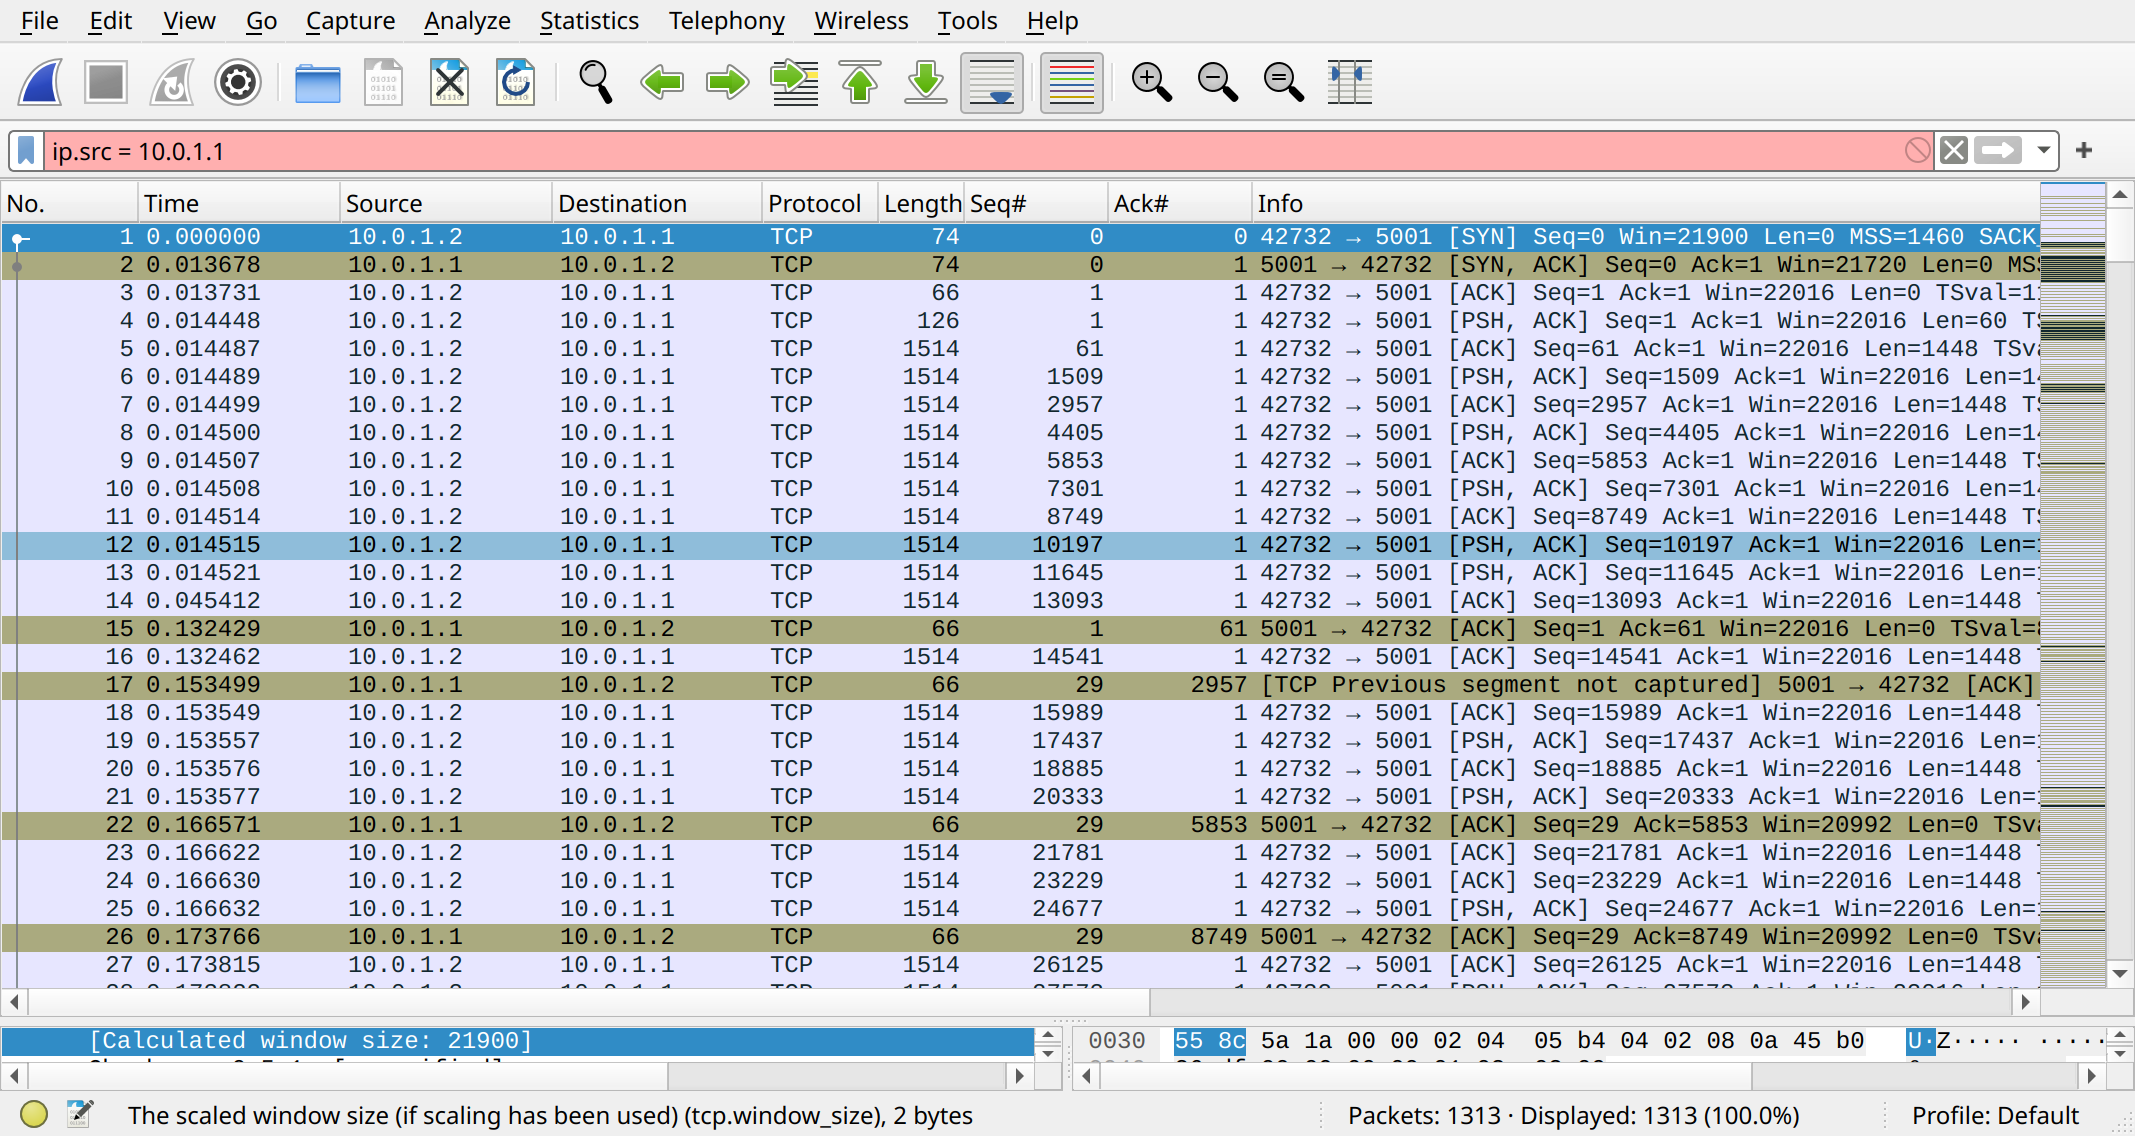
\includegraphics[width=\textwidth]{../reliable/wireshark-tcp-ex2-hi-dir}}%
};
\path (0, 0) rectangle (14.5, -7); % for bounding box
%\draw[overlay,help lines] (0, 0) grid (14, -8);
%\draw[overlay,help lines,dotted] (0, 0) grid[step=0.2] (14, -8);
\begin{visibleenv}<2-3>
\path[draw,red,very thick] (0, -1.5) rectangle (13.9, -2.125);
\node[red,overlay box,anchor=north,align=left] (c setup) at (6.95, -2.125) {
    connection setup, no data transferred 
};
\end{visibleenv}
\only<3>{\spy[rectangle,width=5cm,height=2.5cm,magnification=2] on (7.45, -1.7) in node at (12, 0);}
\begin{visibleenv}<3>
\node[overlay,overlay box,font=\small,anchor=east,align=left] at (9.5, -.5) {
    server+client sequence numbers \\
    advance by 1 to indicate where in setup
};
\end{visibleenv}
\begin{visibleenv}<4>
\path[draw,red,very thick] (0, -1.7) rectangle (13.9, -1.9);
\path[draw,red,very thick] (0, -4.2) rectangle (13.9, -4.39);
\path[draw,red,very thick] (0, -4.55) rectangle (13.9, -4.75);
\path[draw,red,very thick] (0, -5.5) rectangle (13.9, -5.75);
\path[draw,red,very thick] (0, -6.25) rectangle (13.9, -6.45);
\node[overlay box,align=left,anchor=north] at (6.95, -2.5) {
    connection is bidirectional \\
    from now, using olive color to show `backwards' packets
};
\end{visibleenv}
\only<5-6>{\spy on (7.25, -2.3) in node at (10, -1);}
\only<5-6>{\spy on (8, -4.3) in node at (12, -6);}
\begin{visibleenv}<5-6>
\path[draw,red,very thick] (6.55, -2.25 + .2) rectangle (7.5, -2.45 + .2);
    \node[overlay box,text=red,anchor=east,align=left] at (6.55, -2.35) {
        data packet with \\
        client bytes 1--60
    };
\path[draw,red,very thick] (7.55, -4.2) rectangle (8.5, -4.4);
    \node[overlay box,text=red,anchor=east,align=left] at (6.55, -4.3) {
        acknowledgement of \\
        client bytes up to 60
    };
\end{visibleenv}
\begin{visibleenv}<6>
\path[draw,red,very thick] (0, -2.25) rectangle (1.9, -2.45);
\path[draw,red,very thick] (0, -4.2) rectangle (1.9, -4.4);
\path[draw,red,dotted,double,ultra thick] (1, -2.45) -- (1, -4.2) node[midway,font=\small,fill=white,fill opacity=0.957,text=red,text opacity=1.0] {118 ms};
\end{visibleenv}
\begin{visibleenv}<7>
\path[draw,red,very thick] (12.6, -4.15) rectangle (13.3, -4.4);
\path[draw,red,very thick] (6.55, -4.2) rectangle (7.55, -4.4);
\path[draw,red,very thick] (6.55, -4.55) rectangle (7.55, -4.75);
\path[draw,red,very thick] (8.5, -4.55) rectangle (12, -4.75);
\only<7>{\spy[rectangle,width=10cm,magnification=1.5,height=1cm] on (10, -4.5) in node};
    \node[overlay box,text=red,anchor=south,align=left] at (6.55, -3.7) {
        jumps from server byte 0 to server byte 28 \\
        with no data sent \\
        wireshark IDs as missing packet
    };
% FIXME:  hilite len =0 and seq # 29
% FIXME: note missing data packet with bytes 1--28
% FIXME: screenshot scrolled down showing that
\end{visibleenv}
\end{tikzpicture}
\end{frame}

\begin{frame}[fragile]{a TCP connection}
\tikzset{
    overlay box/.style={fill=white,fill opacity=0.95},
}
\begin{tikzpicture}[
    spy using outlines={%
        rectangle,magnification=1.5,height=1cm,width=10cm,connect spies,%
        every spy on node/.append style={very thick},%
        ultra thick,%
    }
]
\node[overlay,anchor=north west,inner sep=0mm] (base) at (0, 0) {%
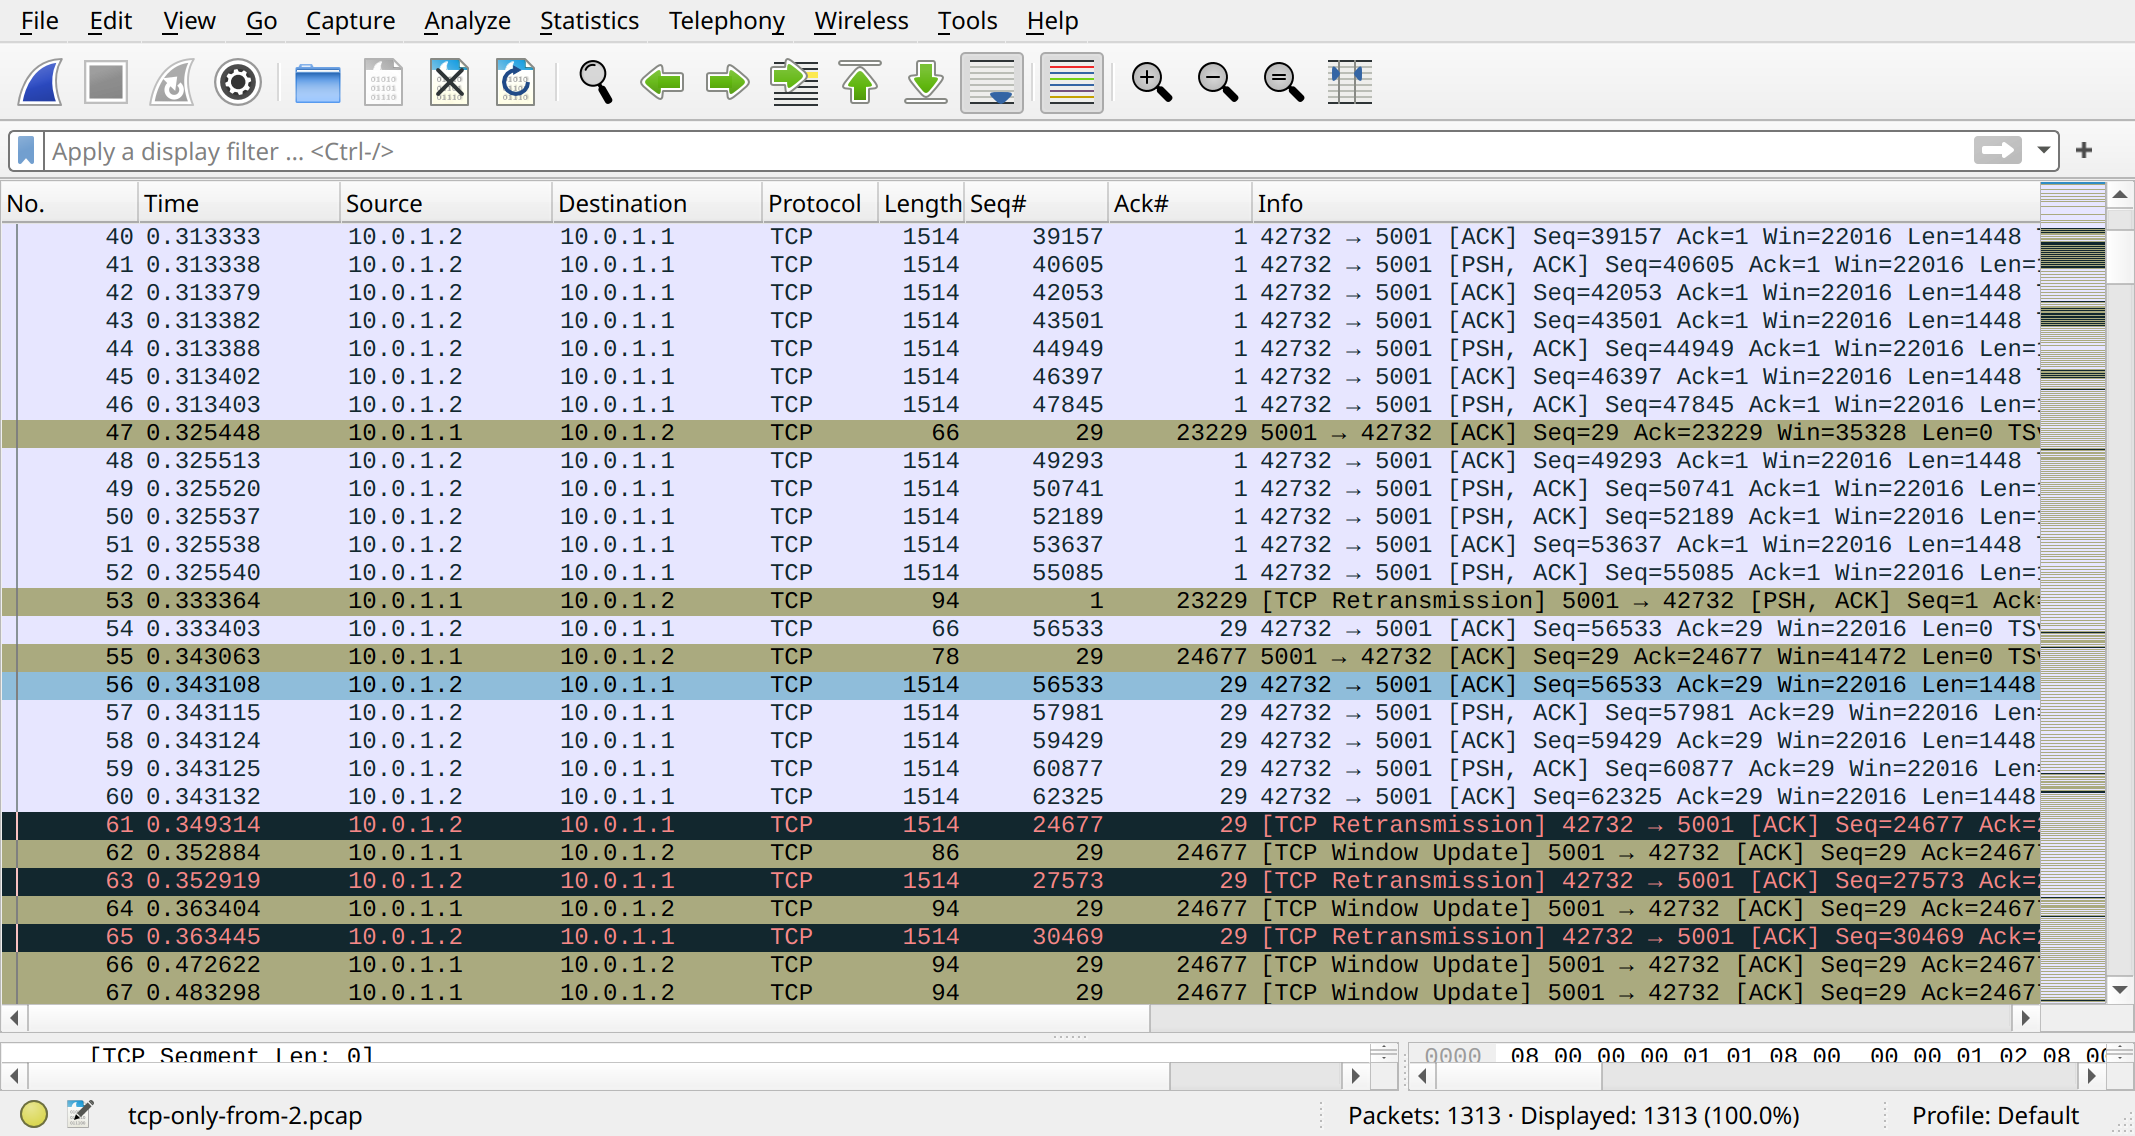
\includegraphics[width=\textwidth]{../reliable/wireshark-tcp-ex2-scrolled-server-retrans}%
};
\path (0, 0) rectangle (14.5, -7); % for bounding box
\spy on (10, -4.0) in node;
    \node[overlay box,text=red,anchor=south,align=left] at (6.55, -3.5) {
        scrolling down reveals retransmission later
    };
    \node[overlay box,text=black,font=\small,anchor=north,align=left] at (6.55, -4.5) {
        wireshark knows it's retransmission because \\
        sequence number sent by server went backwards
    };
\end{tikzpicture}
\end{frame}

\begin{frame}{first data packet}
\begin{tikzpicture}
\tikzset{
    overlay box/.style={fill=white,fill opacity=0.95},
}
\node[overlay,anchor=north west,inner sep=0mm] (base) at (0, 0) {%
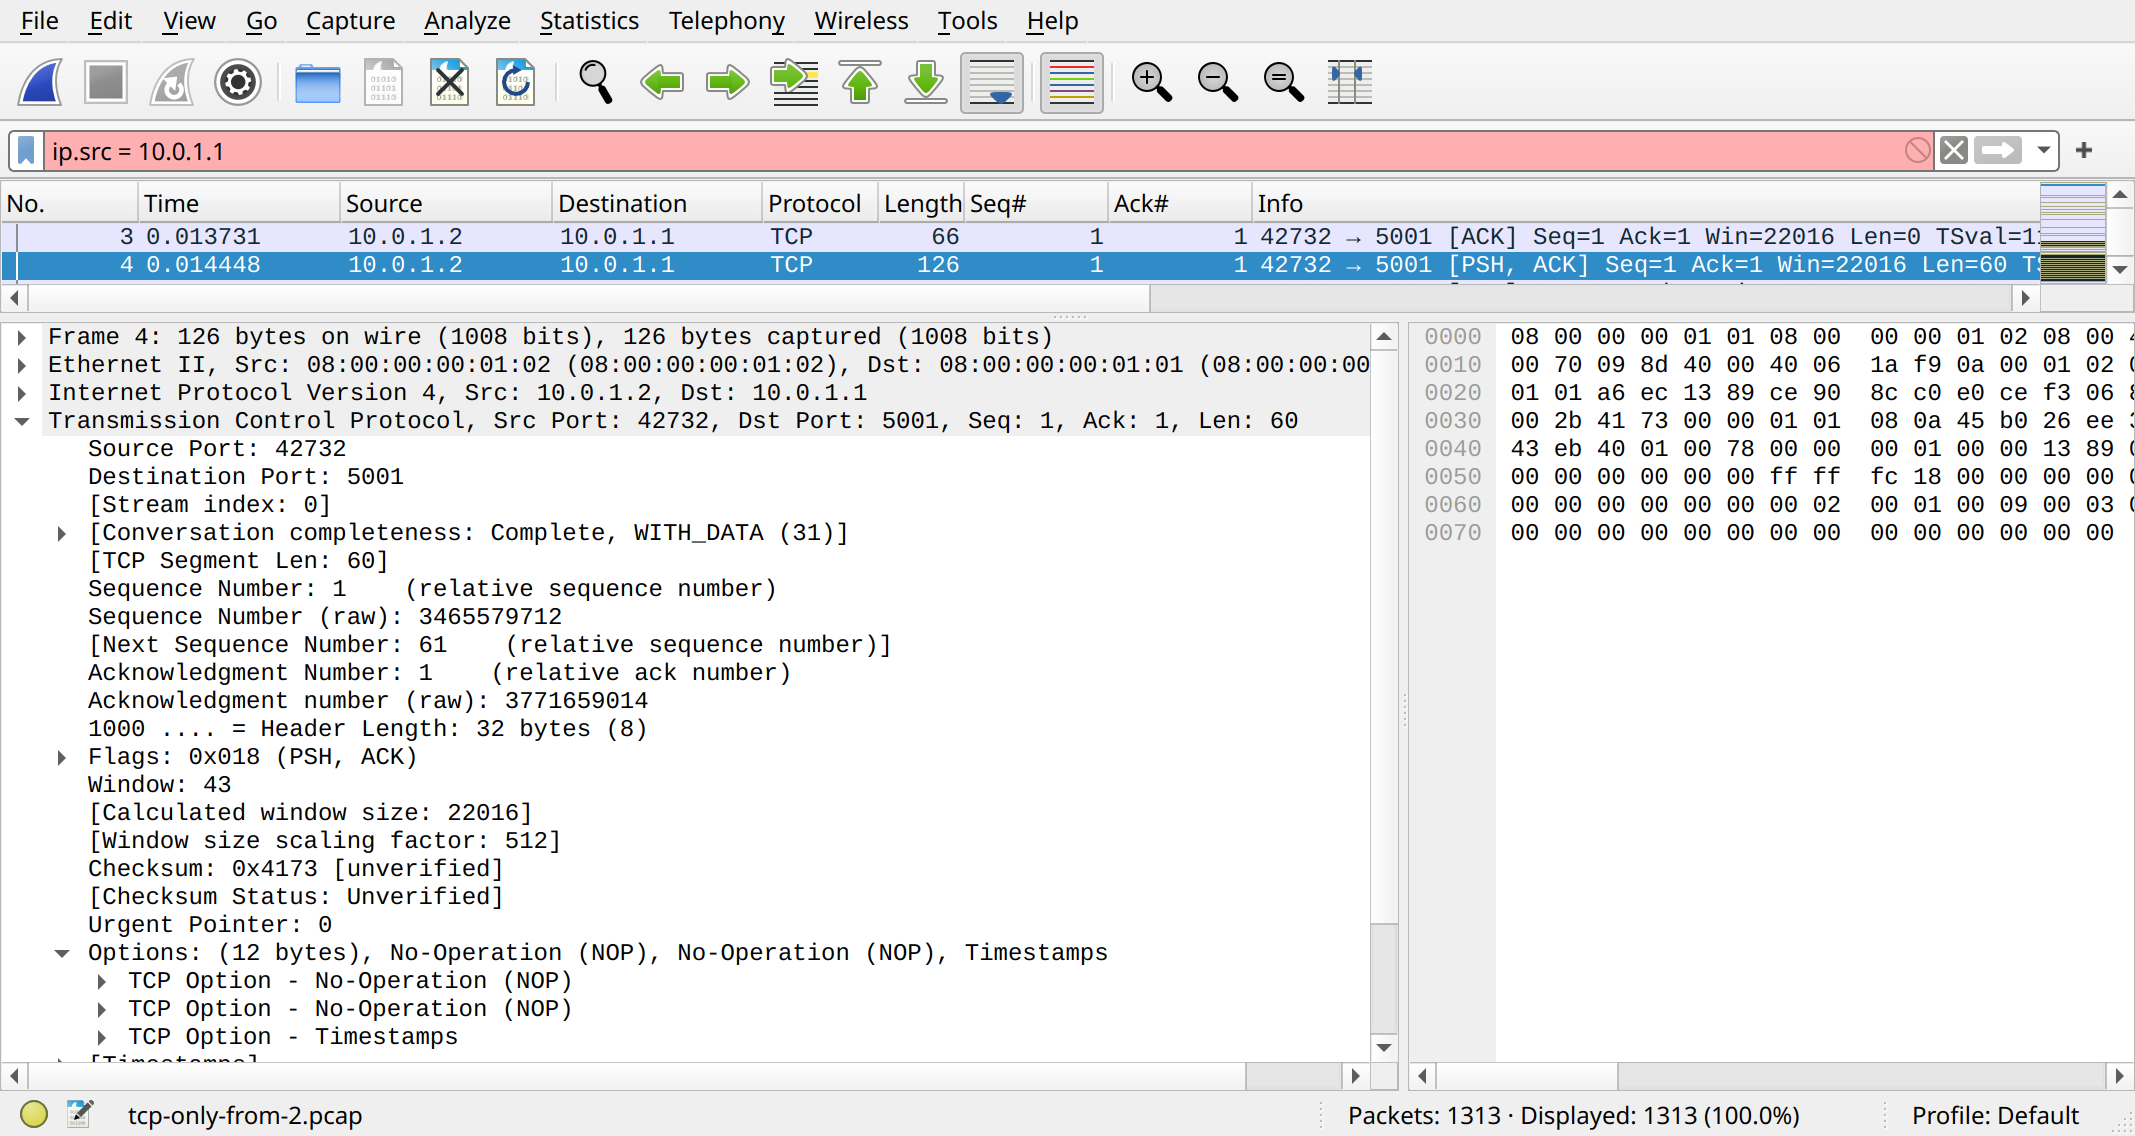
\includegraphics[%
    width=\textwidth,%
    % left bottom right top
    trim={0.5cm 2cm 20cm 10cm},clip,%
]{../reliable/wireshark-tcp-ex2-firstdata}%
};
\path (0, 0) rectangle (14.5, -7); % for bounding box
\draw[violet,overlay,help lines] (0, 0) grid (14, -8);
\draw[violet,overlay,help lines,dotted] (0, 0) grid[step=0.2] (14, -8);
%\spy[overlay,rectangle,magnification=1.7,height=7.5cm,width=10cm] on (3, -5) in node at (9, -3.5);
\begin{visibleenv}<2>
    \draw[red,very thick] (0.65, -2.45) rectangle (3.5, -2.75);
    \node[overlay box,text=red,anchor=west,align=left] at (3.5, -2.6) {
        not actually part of header \\
        computed using length from lower layer
    };
\end{visibleenv}
\begin{visibleenv}<3>
    \draw[red,very thick] (0.65, -2.75) rectangle (8.2, -3.25);
    \node[overlay box,text=red,anchor=north west,align=left] at (0.65, -3.25) {
        sequence numbers in header don't start at 0 \\
        wireshark converts to 0-based indices
    };
\end{visibleenv}
\begin{visibleenv}<4>
    \draw[red,very thick] (0.65, -2.75) rectangle (8.2, -3.55);
    \node[overlay box,text=red,anchor=north west,align=left] at (0.65, -3.55) {
        sequence number is \textit{first} byte being sent \\
        need to use segment length to know last byte's number \\
        (= what to ACK if receiving this)
    };
\end{visibleenv}
\begin{visibleenv}<5>
    \draw[red,very thick] (0.65, -3.55) rectangle (7.3, -4);
    \node[overlay box,text=red,anchor=north west,align=left] at (0.65, -4) {
        ack number indicates received start-of-connection stuff \\
        and nothing else (in case server sent something)
    };
\end{visibleenv}
\begin{visibleenv}<6>
    \draw[red,very thick] (0.65, -4.3) rectangle (3.85, -4.6);
    \node[overlay box,text=red,anchor=north west,align=left] at (0.65, -4.6) {
        PSH = no more data right now \\
        ACK = acknowledgment number is valid 
    };
\end{visibleenv}
\begin{visibleenv}<7>
    \draw[red,very thick] (0.65, -4.55) rectangle (5.15, -5.35);
    \node[overlay box,text=red,anchor=south west,align=left] at (0.7, -4.5) {
        window scaling option in use \\
        (scaling factor only sent in connection setup)
    };
\end{visibleenv}
\begin{visibleenv}<8>
    \draw[red,very thick] (0.65, -6.1) rectangle (10.3, -7.2);
    \node[overlay box,text=red,anchor=south west,align=left] at (0.7, -6.0) {
        no-operation options used to make TCP header size multiple of 4
    };
\end{visibleenv}
\end{tikzpicture}
\end{frame}

\begin{frame}{sequence numbers graph}
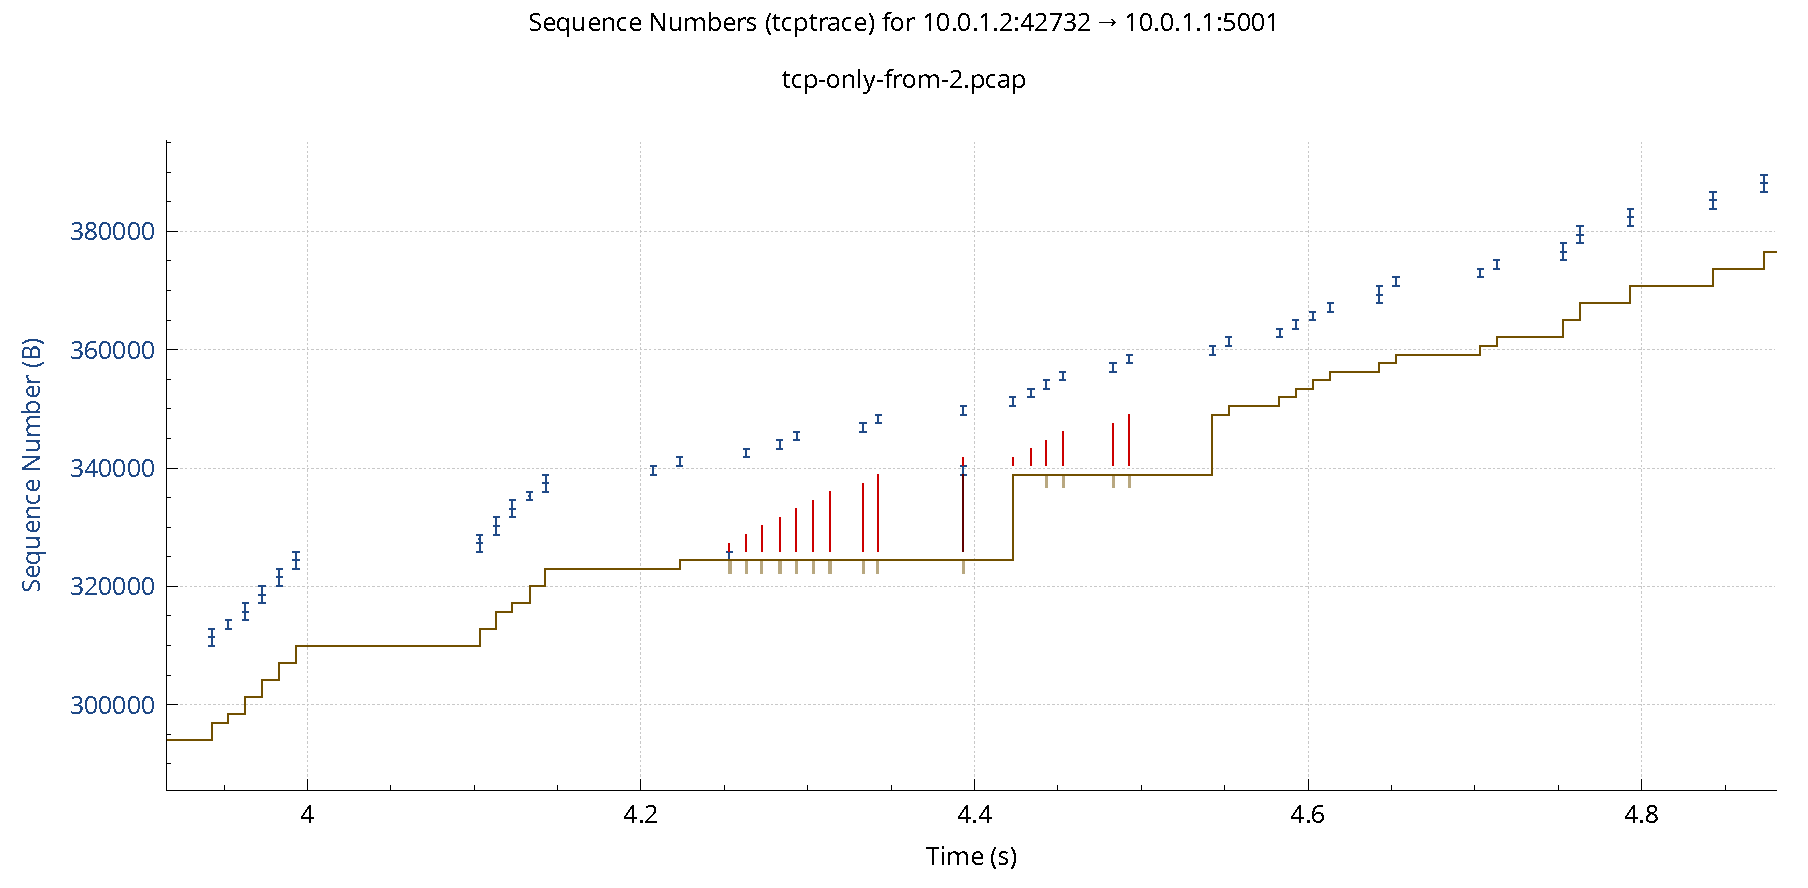
\includegraphics[width=\textwidth]{../reliable/tcptrace-example2}
% FIXME: line at bottom = acknowledgment number from server
% FIXME: blue "I"s = data packets sent
% FIXME: notches on acknowledgment line = duplicate acknowledgments
% FIXME: red lines = selective acknowledgment info
% FIXME: note --- sending new packets triggered by ACK
    % and this is observed from the client
    % so each blue line matches a red line
% FIXME: note slowdown due to congestion
\end{frame}

\begin{frame}{reading thigs graph}
    \begin{itemize}
    \item bottom line = last ack number
    \item notches on bottom line = duplicate acks
    \item red lines = selective ACK info
    \end{itemize}
\end{frame}

\begin{frame}{diff. timing in opposite direction}
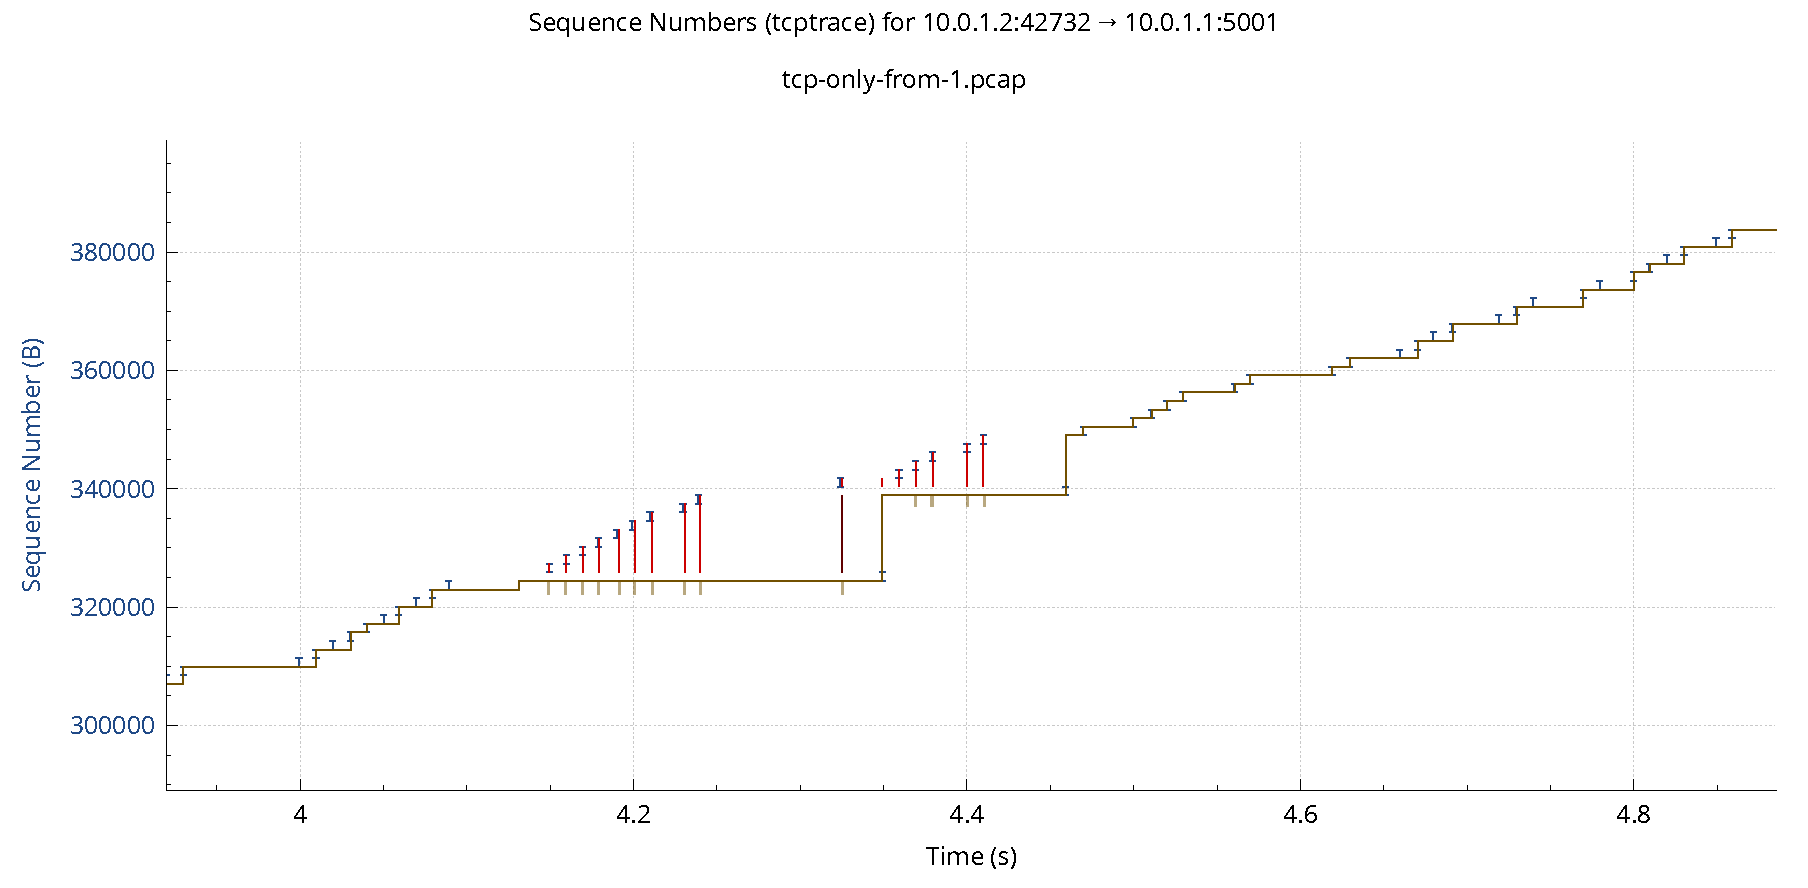
\includegraphics[width=\textwidth]{../reliable/tcptrace-example2-oppdir}
% FIXME: note different timing
\end{frame}



\section{switched networks}

\usetikzlibrary{arrows.meta,calc,shapes}
\providecommand{\computer}{%
    
\includegraphics[width=1cm]{../common/Noun_project_216.pdf}
}
\providecommand{\switch}{%
    
\includegraphics[width=0.9cm]{../common/fig-switch.pdf}
}
\providecommand{\router}{%
    
\includegraphics[width=0.9cm]{../common/fig-router.pdf}
}

\begin{frame}{recall: multi-access media}
\begin{tikzpicture}
\tikzset{
    connect/.style={draw,very thick,arrows={Latex-Circle[width=0.3cm,length=0.3cm]},
        alt=<2>{arrows={Latex-Circle[width=0.3cm,length=0.3cm,red]}}},
    computer/.style={inner sep=0mm,outer sep=0mm,execute at begin node={\computer}},
}
\draw[line width=1mm] (-5,-1.5) coordinate (wire start) -- (5, 1.5) coordinate (wire end);
\foreach \x/\d in {0/5cm,45/4cm,90/3cm,135/4cm,180/5cm,225/4cm,270/3cm,315/4cm} {
    \node[computer] (c-\x) at (\x:\d) {};
    \coordinate (connect-\x) at ($(wire start)!(c-\x.center)!(wire end)$);
    \draw[connect] (c-\x) -- (connect-\x) -- ([turn]0:.1cm);
}
\begin{visibleenv}<2-3>
\node[anchor=north west,fill=white,draw=black,thick,label={[font=\tiny]south:Ali at gwc.org.uk / Alistair1978 via Wikimedia commons / CC-BY-SA 2.5}] 
    (thicknet) at (4, 3.5) {
    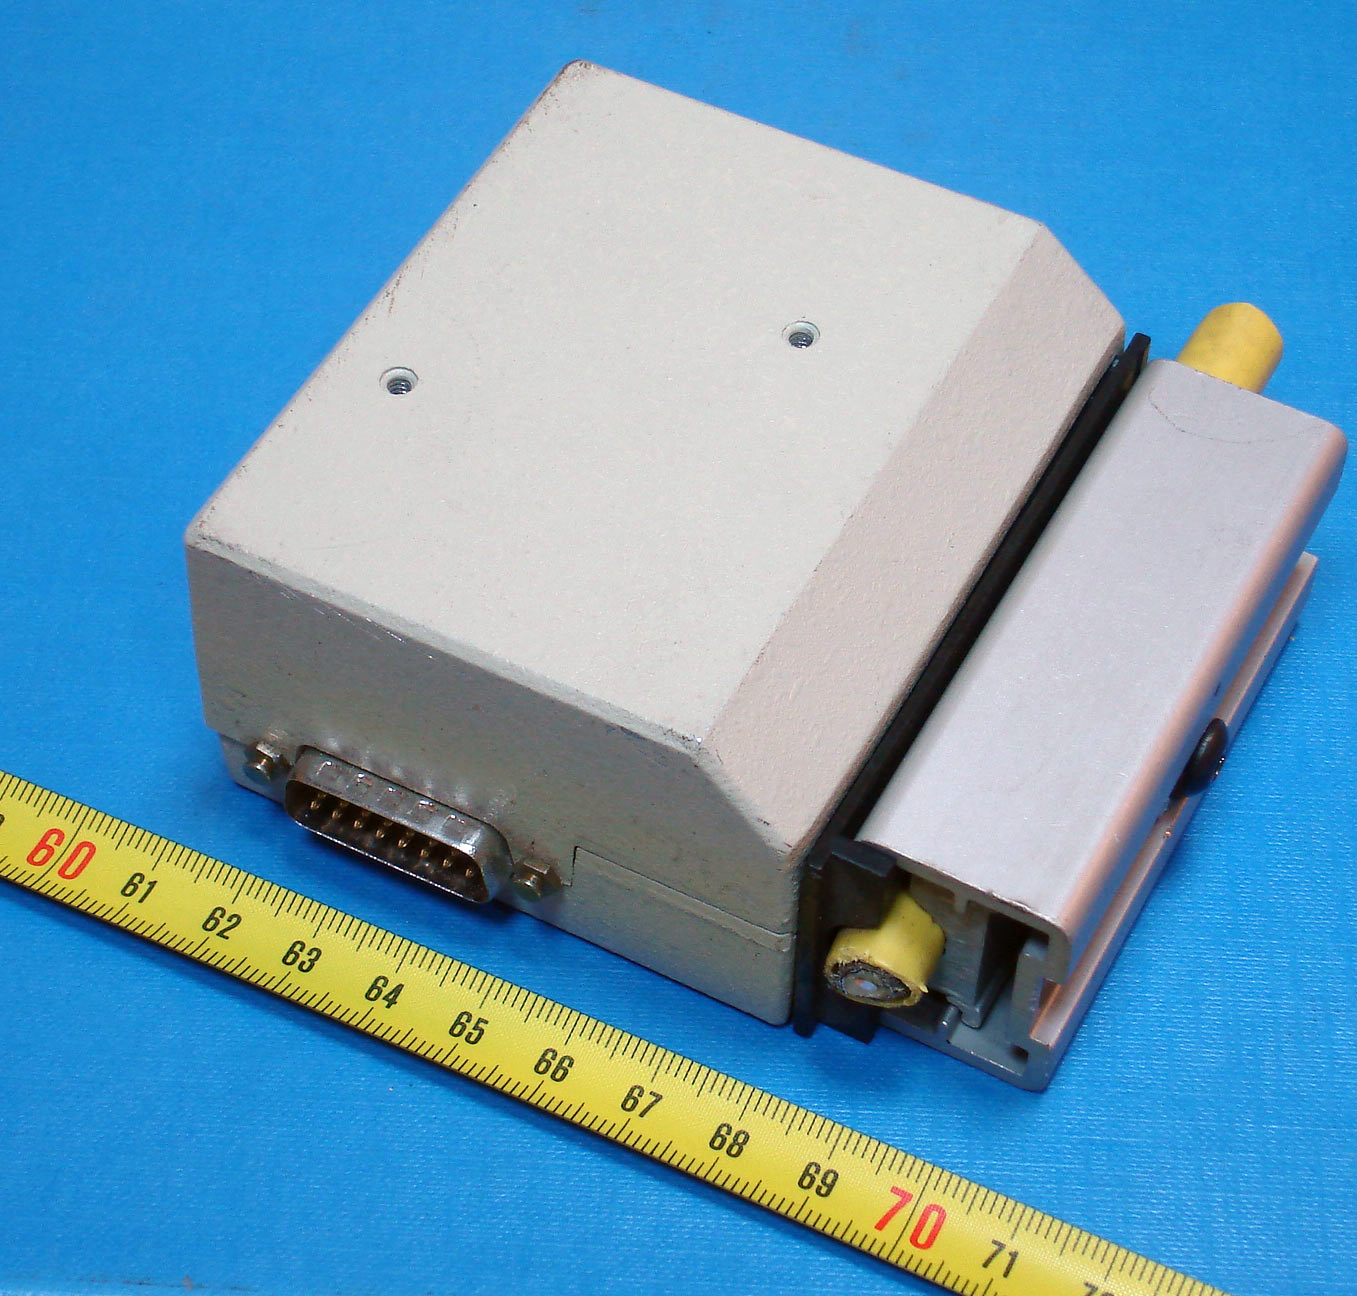
\includegraphics[width=4cm]{../intro/ThicknetTransceiver.jpeg}
};
\end{visibleenv}
\begin{visibleenv}<3>
\node[fill=white,draw=black,thick,anchor=north west] at ([yshift=-0.75cm]thicknet.south west) {
    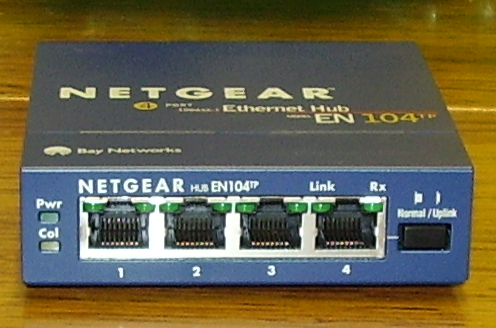
\includegraphics[width=4cm]{../intro/4_port_netgear_ethernet_hub}
};
% FIXME: also fiber splitter
\end{visibleenv}
\end{tikzpicture}
\end{frame}

\begin{frame}{recall: switched network}
\begin{tikzpicture}
\tikzset{
    computer/.style={inner sep=0mm,outer sep=0mm,execute at begin node={\computer}},
    switch/.style={inner sep=0mm,outer sep=0mm,execute at begin node={\switch},
                   alt=<1>{
                       fill=red!10,
                        label={[font=\small,label distance=0mm,text=red]south:`switch'}
                   }},
    connect/.style={draw,very thick,Latex-Latex,alt=<4>{red}},
    connect big/.style={draw,ultra thick,Latex-Latex,alt=<4>{red}},
}
\node[
      cloud,draw,opacity=0.25,very thick,aspect=2,
      minimum width=7cm,minimum height=4cm,
     ] (net-cloud) at (0,0) {};
\foreach \x/\d in {0/5cm,45/4cm,90/3cm,135/4cm,180/5cm,225/4cm,270/3cm,315/4cm} {
    \node[computer] (c-\x) at (\x:\d) {};
}
\node[switch] (s1) at (2,-0.5) {};
\node[switch] (s2) at (-1,0.5) {};
\node[switch] (s3) at (0,-1) {};
\draw[connect] (c-0) -- (s1);
\draw[connect] (c-45) -- (s1);
\draw[connect] (c-315) -- (s1);
\draw[connect] (c-90) -- (s2);
\draw[connect] (c-135) -- (s2);
\draw[connect] (c-180) -- (s2);
\draw[connect] (c-225) -- (s3);
\draw[connect] (c-270) -- (s3);
\draw[connect big] (s1) -- (s2);
\draw[connect big] (s1) -- (s3);
\coordinate (box loc) at (4cm, 4.5cm);
\end{tikzpicture}
\end{frame}

\begin{frame}{hubs and switches}
\begin{tikzpicture}
\node[fill=white,draw=black,thick,label={north:Hub}] (hub) {
    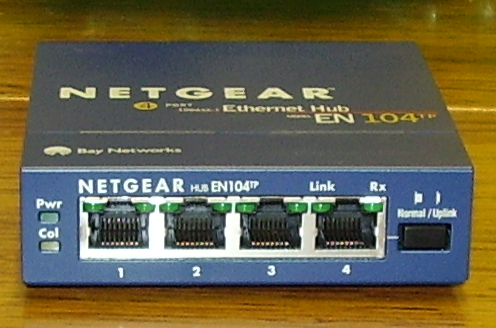
\includegraphics[width=6cm]{../intro/4_port_netgear_ethernet_hub}
};
\node[fill=white,draw=black,thick,anchor=north east,label={north:Switch}] (switch)  at (hub.north west){
    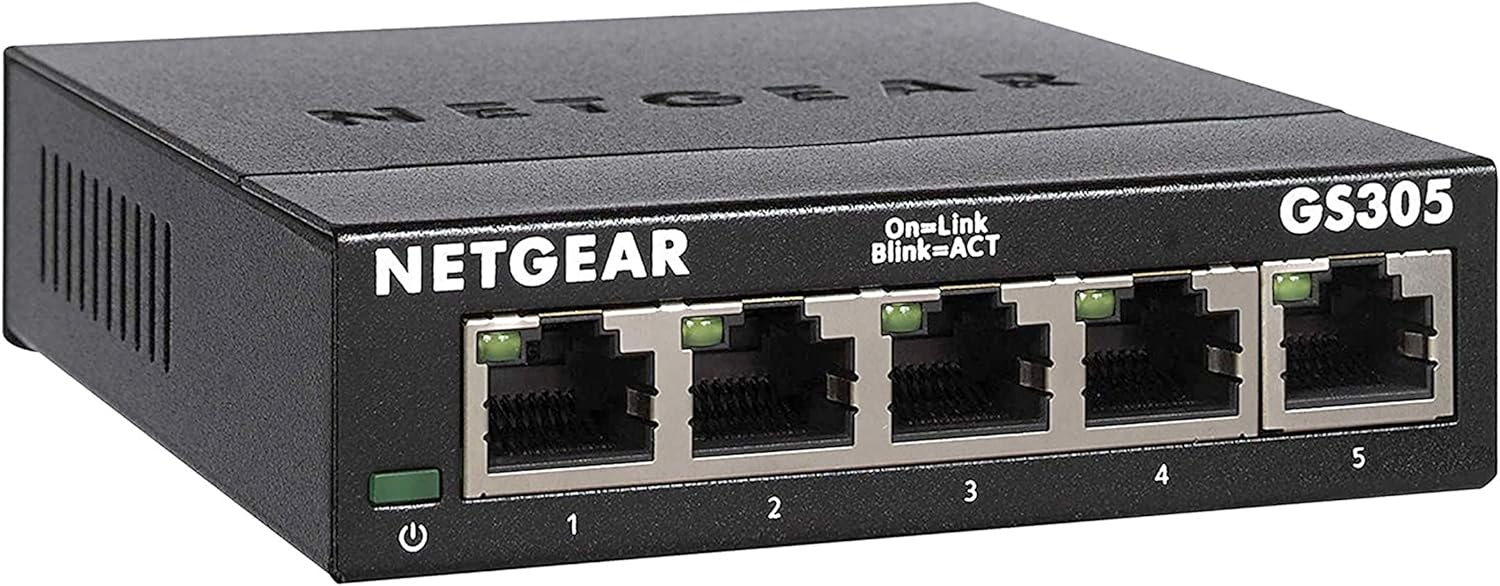
\includegraphics[width=6cm]{../switches/ModernNetgearSwitch}
};
\end{tikzpicture}
\begin{itemize}
\item difference is hidden inside
\item hub: electrically connects hosts --- as if shared wires
\item switch: decides what to send on each output
\end{itemize}
\end{frame}

\begin{frame}{history: multi-access to switched}
    \begin{itemize}
    \item a lot of early networking technology was multi-access
    \item wireless (wifi, cellular) and most home broadband still is
    \vspace{.5cm}
    \item most wired networks are \textit{switched}
        \begin{itemize}
        \item frames mostly directed to correct machine
        \end{itemize}
    \end{itemize}
\end{frame}

\begin{frame}{switching versus routing}
    \begin{itemize}
    \item switches --- forward frames for common network
    \item routers --- forward packets between networks
    \vspace{.5cm}
    \item basically same functionality
    \item differences:
        \begin{itemize}
        \item extra layer for internetwork packets
        \item different mechanism to decide where to forward
        \item switch forwarding typically simpler
        \end{itemize}
    \item will start with simpler switching
    \end{itemize}
\end{frame}



\section{datagrams and Ethernet format}

\usetikzlibrary{patterns}

\begin{frame}{typically sent on Ethernet}
\begin{tikzpicture}
\tikzset{
    box/.style={draw,thick},
    label/.style={font=\small},
    label large/.style={},
    missing/.style={pattern=north west lines},
    start and end/.style={alt=<2>{fill=red!10,text=red}},
    type field/.style={alt=<3-4>{fill=red!10,text=red}},
    destination address/.style={alt=<5-6>{fill=red!10,text=red}},
    source address/.style={alt=<7>{fill=red!10,text=red}},
}
\draw[start and end,box] (4, 0) rectangle (12, -1)
    node[midway,label] {preamble + start marker};
\draw[source address,box] (0, -1) rectangle (6, -2)
    node[midway,label] {source MAC address};
\draw[destination address,box] (6, -1) rectangle (12, -2)
    node[midway,label] {destination MAC address};
\draw[type field,box] (0, -2) rectangle (2, -3)
    node[midway,label] {type};
\draw[box] (2, -2) -- (12, -2) -- (12, -4) -- (0, -4) -- (0, -3) -| cycle;
    \node[label large] at (6, -3) {data (for next layer)};
\begin{visibleenv}<8>
\draw[red,ultra thick] (2, -2) -- (2, -3);
\draw[box,red,ultra thick,fill=white] (4.5, -3) rectangle (11.5, -4) 
    node[midway,label] {sometimes extra stuff (``tags'')};
\end{visibleenv}
\draw[box] (0, -4) rectangle (4, -5) node[midway,label] {checksum};
\draw[start and end,box,missing] (4, -4) rectangle (12, -5)
    node[midway,label,fill=white] {`interpacket gap'};
\draw[start and end,box,missing] (0, -5) rectangle (4, -6);
\begin{visibleenv}<2>
\node[align=left,draw=red,ultra thick,fill=white] at (6, -3) {
    explicit start marker \\
    end indicated by `gap' between signals
};
\end{visibleenv}
\begin{visibleenv}<3>
\node[align=left,draw=red,ultra thick,fill=white] at (8, -3) {
    type field indicates which next layer in use \\
    often varies on frame-by-frame basis \\
};
\end{visibleenv}
\begin{visibleenv}<4>
\node[align=left,draw=red,ultra thick,fill=white] at (8, -3) {
    actually \texttt{type/length} for historical reasons \\
    but most commonly used for type these days
};
\end{visibleenv}
\begin{visibleenv}<5>
\node[align=left,draw=red,ultra thick,fill=white] at (6, -4) {
    destination address indicates who frame is for \\
    present regardless of whether switching is in use \\
    ~ \\
    each host \myemph{filters} out frames for `wrong' destination address
};
\end{visibleenv}
\begin{visibleenv}<6>
\node[align=left,draw=red,ultra thick,fill=white] at (6, -4) {
    since destination address always present \\
    as last resort, switches can send every frame to everyone \\
    ~ \\
    will still work, just much less efficient
};
\end{visibleenv}
\begin{visibleenv}<7>
\node[align=left,draw=red,ultra thick,fill=white] at (6, -4) {
    who the frame came from \\
    gives `return address' for sending replies \\
    ~ \\
    will also be used by switches
};
\end{visibleenv}
\end{tikzpicture}
\end{frame}

\begin{frame}{MAC addresses}
    \begin{itemize}
    \item MAC [media access control] addresses
    \item used by Ethernet, Wifi, and lots of other protocols
    \item 48-bit number written in hex: \texttt{01:23:45:67:89:AB}
        \begin{itemize}
        \item (sometimes seperated with \texttt{-} instead of \texttt{:})
        \end{itemize}
    \item assigned by IEEE to networking manufacturers in blocks
        \begin{itemize}
        \item Institution of Electrical and Electronics Engineers
        \item example: \texttt{00:02:B3:}\ldots, \texttt{00:03:47:}\ldots, (and many more) for Intel
        \end{itemize}
    \vspace{.5cm}
    \item individual addresses hard-coded in networking hardware
        \begin{itemize}
        \item uniquely identify port/device
        \end{itemize}
    \end{itemize}
\end{frame}

\begin{frame}{special MAC addresses}
    \begin{itemize}
    \item \texttt{00:00:00:00:00:00} (all zeroes)
    \item \texttt{FF:FF:FF:FF:FF:FF} (all ones), \texttt{FF:}\ldots
        \begin{itemize}
        \item special destination meaning ``send to everyone'' (on this network)
        \item called \textit{broadcast}
        \end{itemize}
    \item \texttt{01:80:C2:}\ldots, \texttt{33:33:}\ldots, (and some more)
        \begin{itemize}
        \item special destinations representing multiple receivers
        \item example: `all IPv6 routers on this network' (\texttt{33:33:00:00:00:02})
        \item called \textit{multicast}
        \end{itemize}
    \end{itemize}
\end{frame}

\begin{frame}{larger MAC addresses}
    \begin{itemize}
    \item IEEE now calls MAC address EUI-48 (48-bit Extended Unique Identifier)
    \vspace{.5cm}
    \item also created EUI-64, with 64-bit addresses
        \begin{itemize}
        \item way of mapping EUI-48s to EUI-64s
        \item turns out 48 bits might have been low
        \end{itemize}
    \item I'm not sure what status is on switching to 64-bit addresses
        \begin{itemize}
        \item IEEE 802.15.4 (used in ZigBee, 6LoWPAN, some others) uses EUI-64
        \item I don't know other local network protocols that do
        \end{itemize}
    \end{itemize}
\end{frame}


% FIXME: example in wireshark

\subsection{versus virtual circuits}

\begin{frame}{datagram idea}
    \begin{itemize}
    \item can always send something to anyone on network
        \begin{itemize}
        \item just put destination MAC in frame
        \end{itemize}
    \item no need for reservations/`connections'/etc.
        \begin{itemize}
        \item not like the interface you've seen with [TCP] sockets
        \end{itemize}
    \vspace{.5cm}
    \item not the only model for networks (and internetworks)
    \end{itemize}
\end{frame}

\begin{frame}{virtual circuit}
    \begin{itemize}
    \item other model: virtual circuit
    \item two machines setup a `circuit'
        \begin{itemize}
        \item some sort of `special' messages to do this
        \end{itemize}
    \item switches/routers \myemph{reserve resources} for circuit
        \begin{itemize}
        \item ``gaurenteed'' bandwidth
        \end{itemize}
    \item transmitted data must be part of estabished circuit
    \vspace{.5cm}
    \item example: ATM (Asynchronous Transfer Mode)
        \begin{itemize}
        \item used (?historically?) by some telephone networks
        \end{itemize}
    \end{itemize}
\end{frame}


\section{switch architecture}

\subsection{now programmable}
\begin{frame}{an annoyance}
    \begin{itemize}
    \item traditionally, switches/routers have been `fixed function' specialized hardware
    \vspace{.5cm}
    \item special hardware needed for multigigabit performance
    \item limited configuration options
    \item usually non-automated configuration
        \begin{itemize}
        \item login to each managed switch/router to change settings
        \item no standardization for configuration across vendors
        \end{itemize}
    \item little visibility into internal design
        \begin{itemize}
        \item even though switches/routers often running complicated programs
        \end{itemize}
    \end{itemize}
\end{frame}

\begin{frame}{the historical situation}
    \begin{itemize}
    \item let's say I want to design a new extension to Ethernet
    \vspace{.5cm}
    \item historical options if want to test/deploy it\ldots
        \begin{itemize}
        \item implement it in slow/low-capacity software/FPGA switch
        \item convince switch HW company to implement it + release new version of switches
        \item contort my modification to fit with switch features not intended for this use
            \begin{itemize}
            \item example: using VPN support to change path of frames on network
            \end{itemize}
        \end{itemize}
    \end{itemize}
\end{frame}



\subsection{control v dataplane}
\begin{frame}{software defined networking (SDN)}
    \begin{itemize}
    \item movement toward \textit{programmable} networks
    \vspace{.5cm}
    \item ``software-defined''
        \begin{itemize}
        \item rules about how network works defined in ``normal'' software
        \end{itemize}
    \end{itemize}
\end{frame}

\begin{frame}{control plane and data plane}
    \begin{itemize}
    \item control plane
        \begin{itemize}
        \item decides \textit{how} to handle traffic
        \item ``slow path'', where complicated decisions are
        \end{itemize}
    \item data plane
        \begin{itemize}
        \item actually implements the decisions made by the control plane
        \item ``fast path'', implementing simple rules
        \end{itemize}
    \vspace{.5cm}
    \item probably what switches did internally before SDN was a thing
    \end{itemize}
\end{frame}

\begin{frame}{separate control/data plane}
    \begin{itemize}
    \item one SDN key idea: separate control and data plane
    \item allow new \myemph<2>{vendor-neutral} implementations of control plane
        \begin{itemize}
        \item requires standard interface for programming data plane
        \item most prominent example: OpenFlow
        \end{itemize}
    \item easily allows for central `control plane' server
        \begin{itemize}
        \item instead of separate control plane running on each switch/router
        \end{itemize}
    \end{itemize}
\end{frame}


\subsection{P4 dataplane}
\begin{frame}{P4}
    \begin{itemize}
    \item P4 --- programming langauge for data planes
    \item intended to be compiled to run on fast switches
    \item includes `runtime' defining how control plane configures data plane
    \end{itemize}
\end{frame}

\begin{frame}{future P4 assignment}
    \begin{itemize}
    \item given: 
        \begin{itemize}
        \item simple P4 switch that doesn't know where to direct frames
        \item simpler controller (in Python) that configures switch
        \item simulated 4-machine network in VM
        \end{itemize}
    \item your task will be:
        \begin{itemize}
        \item have controller write static configuration to direct to right place
        \item modify data plane to send information to control plane
        \item have controller change configuration based on info from data plane
        \end{itemize}
    \item (we'll discuss more details later)
    \end{itemize}
\end{frame}

\begin{frame}{P4 switch architecture}
\begin{tikzpicture}
\foreach \x in {1,2,3,4} {
    \begin{scope}[yshift=\x cm,y=0.9cm]
        \draw[thick] (0, 0) rectangle (2, 1);
        \draw[ultra thick,-Latex] (-1, .5) -- (0, .5);
        \foreach \off in {1,1.2,1.4,1.6,1.8} {
            \draw[thick] (\off, 0) -- (\off, 1);
        }
    \end{scope}
}
\tikzset{
    box/.style={draw,thick},
    box label/.style={font=\small},
};
\foreach \x/\name in {3/parser,5/ingress,7/deparser} {
    \draw[box] (\x, 1) coordinate (\name in base) rectangle ++(1.6, 2) coordinate (name other base) node[midway,box label] (\name label) {\name};
    \draw[box] (\x + 1.4, 1) |- (\x - .2, .8) |- (\x, 1.8); 
    \draw[box] (\x + 1.2, 1) |- (\x - .4, .6) |- (\x, 1.6); 
}
\foreach \x/\name in {11/parser,13/egress,15/deparser} {
    \draw[box] (\x, 1) coordinate (\name out base) rectangle ++(2, 2) coordinate (name other base) node[midway,box label] (\name label) {\name};
    \draw[box] (\x + 1.4, 1) |- (\x - .2, .8) |- (\x, 1.8); 
    \draw[box] (\x + 1.2, 1) |- (\x - .4, .6) |- (\x, 1.6); 
}
\end{tikzpicture}
\end{frame}

% FIXME:
    % example parser + deparser program
        % idea of copying from buffer to control structure
    % example match-pipeline
        % show table lookup
        % show standard_metadata
    
    % example configuration


\subsection{P4 controlplane}

\begin{frame}<1>[label=controlToC]{P4: control plane}
    \begin{itemize}
    \item P4 control plane is a program
    \vspace{.5cm}
    \item sends commands to one or more switches:
        \begin{itemize}
        \item \myemph<2>{load P4 program into data plane}
        \item \myemph<3>{set table entries}
        \item \myemph<4>{configure multicast groups}
        \item \myemph<5>{receive frames to process them}
        \end{itemize}
    \end{itemize}
\end{frame}

\begin{frame}{aside: wrappers}
    \begin{itemize}
    \item I'll show code from a P4 controller for upcoming assignment
    \item written in Python, using custom library to make things convenient
    \item works with softawre based reference switch
    \vspace{.5cm}
    \item no requirement to use Python or other specific language
        \begin{itemize}
        \item controller sends commands over network/IPC to data plane
        \end{itemize}
    \item real raw code has more boilerplate/etc.
    \item probably several things different for hardware-based switches
    \end{itemize}
\end{frame}

\againframe<2>{controlToC}

\begin{frame}[fragile]{P4: loading P4 program}
\providecommand{\vemphA}[1]{\myemph<2>{#1}}
\providecommand{\vemphB}[1]{\myemph<3>{#1}}
\providecommand{\vemphC}[1]{\myemph<4>{#1}}
\providecommand{\vemphD}[1]{\myemph<5>{#1}}
\begin{Verbatim}[fontsize=\small,commandchars=\\@~]
p4info_helper =  ....
switch = ....
\vemphA@switch.MasterArbitrationUpdate()~
switch.\vemphB@SetForwardingPipelineConfig~(
    p4info=p4info_helper.p4info,
    \vemphC@bmv2_json_file_path=bmv2_file_path~
)
\end{Verbatim}
\begin{tikzpicture}[overlay,remember picture]
\tikzset{
    box/.style={
        align=left,
        draw=red,
        fill=white,
        ultra thick,
        anchor=north,
        at={([yshift=-1cm]current page.center)},
    },
}
    \begin{visibleenv}<2>
    \node[box] {
        swtich supports having primary + backup controller, \\
        so need to indicate this is primary controller now \\
    };
    \end{visibleenv}
    \begin{visibleenv}<3>
    \node[box] {
        ``forwarding pipeline'' = dataplane
    };
    \end{visibleenv}
    \begin{visibleenv}<4>
    \node[box] {
        P4 code compiled to file to load, specified here
    };
    \end{visibleenv}
\end{tikzpicture}
\end{frame}

\againframe<3>{controlToC}

\begin{frame}[fragile]{P4: setting table entries}
\providecommand{\vemphA}[1]{\myemph<2>{#1}}
\providecommand{\vemphB}[1]{\myemph<3>{#1}}
\providecommand{\vemphC}[1]{\myemph<4>{#1}}
\providecommand{\vemphD}[1]{\myemph<5>{#1}}
\begin{Verbatim}[fontsize=\small,commandchars=\\@~]
\vemphD@write_or_overwrite_table_entry~(
    \vemphA@p4info_helper=p4info_helper, switch=switch,~
    table_name='\vemphB@MyIngress.mac_dst_exact~',
    match_fields={
        'hdr.ethernet.dstAddr': \vemphC@some_address~,
    },
    action_name='forward_to',
    action_params={'port': port},
)
\end{Verbatim}
\begin{tikzpicture}[overlay,remember picture]
\tikzset{
    box/.style={
        align=left,
        draw=red,
        fill=white,
        ultra thick,
        anchor=north,
        at={([yshift=-1cm]current page.center)},
    },
}
    \begin{visibleenv}<2>
    \node[box] {
        p4info\_helper, switch objects created by setup code
    };
    \end{visibleenv}
    \begin{visibleenv}<3>
    \node[box] {
        full name of table, including stage it is defined in
    };
    \end{visibleenv}
    \begin{visibleenv}<4>
    \node[box] {
        match value --- format would be different \\
        if key was \texttt{lpm} or \texttt{ternary} \\
        instead of exact match
    };
    \end{visibleenv}
    \begin{visibleenv}<5>
    \node[box] {
        \texttt{write\_or\_overwrite\_table\_entry} not the `raw' function \\
        (one I wrote based on one P4 tutorial authors wrote) \\
        uses gRPC (remote procedure call) library, which adds some extra steps
    };
    \end{visibleenv}
\end{tikzpicture}
\end{frame}

\againframe<4>{controlToC}
\begin{frame}[fragile]{P4: multicast groups}
\providecommand{\vemphA}[1]{\myemph<2>{#1}}
\providecommand{\vemphB}[1]{\myemph<3>{#1}}
\providecommand{\vemphC}[1]{\myemph<4>{#1}}
\providecommand{\vemphD}[1]{\myemph<5>{#1}}
\begin{Verbatim}[fontsize=\small,commandchars=\\@~]
switch.Write\vemphC@PRE~Entry(
    p4info_helper.buildMulticastGroupEntry(
        \vemphA@multicast_group_id=1~, 
        \vemphB@replicas~=[
            {'egress_port': 1, 'instance': 0},
            {'egress_port': 2, 'instance': 0},
            {'egress_port': 3, 'instance': 0},
            {'egress_port': 4, 'instance': 0},
        ]
    )
)
\end{Verbatim}
\begin{tikzpicture}[overlay,remember picture]
\tikzset{
    box/.style={
        align=left,
        draw=red,
        fill=white,
        ultra thick,
        anchor=north,
        at={([yshift=-1cm]current page.center)},
    },
}
    \begin{visibleenv}<2>
    \node[box] {
        in P4 dataplane code can write \\
        \texttt{standard\_metadata.mcast\_grp = 1} to use this
    };
    \end{visibleenv}
    \begin{visibleenv}<3>
    \node[box] {
        list of ports to output to when group selected \\
        ~ \\
        \texttt{instance} can be inspected by dataplane code \\
        for the egress step
    };
    \end{visibleenv}
    \begin{visibleenv}<4>
    \node[box] {
        PRE = packet replication engine \\
        ~ \\
        supports multicast groups (shown) and ``clone sessions'' (not shown) \\
        (clone sessions make extra copy of packet, \\
        but process original normally)
    };
    \end{visibleenv}
\end{tikzpicture}
\end{frame}

\againframe<5>{controlToC}
\begin{frame}[fragile]{P4: receiving frame}
\providecommand{\vemphA}[1]{\myemph<2>{#1}}
\providecommand{\vemphB}[1]{\myemph<3>{#1}}
\providecommand{\vemphC}[1]{\myemph<4>{#1}}
\providecommand{\vemphD}[1]{\myemph<5>{#1}}
\begin{Verbatim}[fontsize=\small,commandchars=\\@~]
    for item in switch.stream_msg_resp:
        if item.HasField('packet'):
            do_something_with(\vemphA@item.packet.payload~,
                              \vemphB@item.packet.metadata~)
\end{Verbatim}
\begin{tikzpicture}[overlay,remember picture]
\tikzset{
    box/.style={
        align=left,
        draw=red,
        fill=white,
        ultra thick,
        anchor=north,
        at={([yshift=0cm]current page.center)},
    },
}
    \begin{visibleenv}<2>
    \node[box] {
        payload = bytes of frame  \\
        (what would normally be sent on network)
    };
    \end{visibleenv}
    \begin{visibleenv}<3>
    \node[box] {
        extra metadata can be set by dataplane \\
        example: which port packet came from
    };
    \end{visibleenv}
\end{tikzpicture}
\end{frame}


\section{basic Ethernet switching / MAC learning}

\againframe<10>{ethernetFormat}

% FIXME: show before/after wireshark picture form assignment

\usetikzlibrary{arrows.meta,calc,matrix,shapes}
\providecommand{\computer}{%
    
\includegraphics[width=1cm]{../common/Noun_project_216.pdf}
}
\providecommand{\switch}{%
    
\includegraphics[width=0.9cm]{../common/fig-switch.pdf}
}
\providecommand{\router}{%
    
\includegraphics[width=0.9cm]{../common/fig-router.pdf}
}

\begin{frame}{network and switch tables}
\begin{tikzpicture}
\tikzset{
    computer/.style={inner sep=0mm,outer sep=0mm,execute at begin node={\computer}},
    switch/.style={inner sep=0mm,outer sep=0mm,execute at begin node={\switch}},
    connect/.style={draw,very thick,Latex-Latex},
    connect big/.style={draw,ultra thick,Latex-Latex},
    port/.style={pos=0.95,fill=white,circle,draw,inner sep=0mm},
    port beginning/.style={pos=0.05,fill=white,circle,draw,inner sep=0mm},
    mac label/.style={
        visible on=<2->,draw,fill=white,inner sep=1mm,font=\tiny\tt,
        alt=<2>{text=red,draw=red},
    },
    route table/.style={
        matrix of nodes,ampersand replacement=\&,
        column 1/.style={nodes={draw,thick,text width=2.5cm,font=\tiny\tt,text depth=0mm,minimum height=0.5cm,inner sep=1mm}},
        column 2/.style={nodes={draw,thick,text width=.5cm,font=\small\tt,text depth=0mm,minimum height=0.5cm,inner sep=1mm}},
        row 1/.style={nodes={draw=none,font=\small}},
    }
}
\foreach \x/\d/\mc/\dir in {15/8cm/AA/north,45/3cm/BB/north,90/2cm/CC/north,135/3cm/DD/north,180/4cm/EE/north,300/4cm/FF/south} {
    \node[computer,label={[mac label,]\dir:00:11:22:33:44:\small\mc}] (c-\x) at (\x:\d) {};
}
\node[switch,alt=<4>{fill=red!10}] (s1) at (4,-0.5) {};
\begin{visibleenv}<4->
\matrix[route table,alt=<4>{fill=red!10},anchor=north west] (s1 table) at ([xshift=1cm,yshift=.5cm]s1.north east) {
dst MAC addr \& port \\
00:11:22:33:44:\small AA \& 1 \\
00:11:22:33:44:\small BB \& 2 \\
00:11:22:33:44:\small CC \& 4 \\
00:11:22:33:44:\small DD \& 4 \\
00:11:22:33:44:\small EE \& 4 \\
00:11:22:33:44:\small FF \& 3 \\
};
\draw[dotted,thick] (s1.north east) -- (s1 table-2-1.north west);
\draw[dotted,thick] (s1.south east) -- (s1 table-7-1.south west);
\end{visibleenv}
\node[switch,alt=<3>{fill=red!10}] (s2) at (-1,0.5) {};
\begin{visibleenv}<3->
\matrix[route table,alt=<3>{fill=red!10},anchor=north east] (s2 table) at ([xshift=2cm]s2.south west) {
dst MAC addr \& port \\
00:11:22:33:44:\small AA \& 1 \\
00:11:22:33:44:\small BB \& 1 \\
00:11:22:33:44:\small CC \& 2 \\
00:11:22:33:44:\small DD \& 3 \\
00:11:22:33:44:\small EE \& 4 \\
00:11:22:33:44:\small FF \& 2 \\
};
\draw[dotted,thick] (s2.south east) -- (s2 table-2-2.north east);
\draw[dotted,thick] (s2.south west) -- (s2 table-2-1.north west);
\end{visibleenv}
\draw[connect] (c-15) -- (s1) node[port] {1};
\draw[connect] (c-45) -- (s1) node[port] {2};
\draw[connect] (c-300) -- (s1) node[port] {3};
\draw[connect] (c-90) -- (s2) node[port] {2};
\draw[connect] (c-135) -- (s2) node[port] {3};
\draw[connect] (c-180) -- (s2) node[port] {4};
\draw[connect big] (s1) -- (s2) node[port beginning] {4} node [port] {1};
\end{tikzpicture}
\end{frame}

\begin{frame}{constructing switch tables}
    \begin{itemize}
    \item could have system administrator input these by hand
        \begin{itemize}
        \item through an SSH-like interface, probably
        \end{itemize}
    \item works, but error-prone, hard to change, etc.
    \vspace{.5cm}
    \item<2-> alternative: switch should figure it out
    \end{itemize}
\end{frame}

\begin{frame}{MAC learning}
\begin{tikzpicture}
\tikzset{
    route table/.style={
        matrix of nodes,ampersand replacement=\&,
        column 1/.style={nodes={draw,thick,text width=2.5cm,font=\tiny\tt,text depth=1mm,text height=3.5mm,minimum height=0.6cm,inner sep=1mm}},
        column 2/.style={nodes={draw,thick,text width=1cm,font=\small\tt,text depth=1mm,text height=3.5mm,minimum height=0.6cm,inner sep=1mm}},
        row 1/.style={nodes={draw=none,font=\small}},
    }
}
\matrix[label={north:forwarding table},route table,draw,very thick,anchor=north east] (table) {
dst MAC addr \& port \\
|[alt={<5,7>{fill=red!10}}]| \alt<5->{00:11:22:33:44:AA}{~}
    \& |[alt={<5,7>{fill=red!10}}]| \alt<5->{2}{~} ~ \\
|[alt={<8>{fill=red!10}}]| \alt<8->{00:11:22:33:44:FF}{~}
    \& |[alt={<8>{fill=red!10}}]| \alt<8->{3}{~} ~ \\
~ \& ~ \\
~ \& ~ \\
~ \& ~ \\
~ \& ~ \\
|[alt={<2,4>{fill=red!10}}]|  \alt<2->{(default)}{~} 
    \& |[alt={<2,4>{fill=red!10}}]| \alt<2->{ALL*}{~} \\
};
\begin{visibleenv}<3->
\matrix[
    draw,very thick,label={north:incoming frame 1},anchor=north west,tight matrix,
    nodes={text width=8cm,font=\small}
] (pkt 1) at ([xshift=1cm]table.north east) {
    input port=\myemph<5>{2}, output port = \alt<4->{\myemph<4>{all but 2}}{\myemph<3>{???}} \\
    data = {
\begin{tabular}{l}
src=\tt \myemph<5>{00:11:22:33:44:AA} \\ dst=\tt \myemph<2>{00:11:22:33:44:FF} \\
type = IPV4  \\ data = \tt33 45 43 42 \ldots \\
\end{tabular}
} \\
};
\end{visibleenv}
\begin{visibleenv}<6->
\matrix[
    draw,very thick,label={north:incoming frame 2},anchor=north west,tight matrix,
    nodes={text width=8cm,font=\small}
] (pkt 2) at ([yshift=-1cm]pkt 1.south west) {
    input port=\myemph<8>{3}, output port = \alt<7->{\myemph<7>{2}}{???} \\
    data = {
\begin{tabular}{l}
src=\tt \myemph<8>{00:11:22:33:44:FF} \\ dst=\tt \myemph<7>{00:11:22:33:44:AA} \\
type = IPV4  \\ data = \tt34 45 43 42 \ldots \\
\end{tabular}
} \\
};
\end{visibleenv}
\end{tikzpicture}
\end{frame}

% FIXME: picture of network with switch ports labeled
    % FIXME: picture of ideal mac_dst_exact tables for it

% ideal: table of MAC addresses
% note: multiple MAC addresses per port
    % assumption: no loops
% fallback: broadcast

\begin{frame}{fallback option}
    \begin{itemize}
    \item very low quality switch: \\
    send every frame to every \textit{other} port
    \vspace{.5cm}
    \item receivers will check destination
        \begin{itemize}
        \item check dates to history of unswitched (shared medium) ethernet
        \item sending to extra destinations just slow
        \end{itemize}
    \vspace{.5cm}
    \item as optimization: want to only send where interested
    \end{itemize}
\end{frame}



% FIXME: example of using tcpdump/etc. in implementation

\subsection{aside: no loops please}

\usetikzlibrary{arrows.meta,decorations.markings,patterns}

\providecommand{\computer}{%
    
\includegraphics[width=1cm]{../common/Noun_project_216.pdf}
}
\providecommand{\switch}{%
    
\includegraphics[width=0.9cm]{../common/fig-switch.pdf}
}
\providecommand{\router}{%
    
\includegraphics[width=0.9cm]{../common/fig-router.pdf}
}

\begin{frame}[label=noBackwardsQ]{aside: no backwards broadcast}
    \begin{itemize}
    \item recall: broadcast sent to all but incoming port
    \item question: what would happen if we didn't do this?
        \begin{itemize}
        \item multiple may apply
        \end{itemize}
    \end{itemize}
\begin{tabular}{l}
A. might cause host to receive duplicates \\
B. might cause copies sent to non-incoming port to be dropped \\
C. might cause frames sent at same time to be dropped \\
D. might cause frames sent much later to be dropped \\
\end{tabular}
\end{frame}

\begin{frame}[fragile]{loop from backwards broadcast}
\begin{tikzpicture}[remember picture]
\tikzset{
    computer/.style={inner sep=0mm,outer sep=0mm,execute at begin node={\computer}},
    switch/.style={inner sep=0mm,outer sep=0mm,execute at begin node={\switch}},
    connect/.style={draw,very thick,Latex-Latex},
    connect big/.style={draw,ultra thick,Latex-Latex},
    port/.style={pos=0.95,fill=white,circle,draw,inner sep=0mm},
    port beginning/.style={pos=0.05,fill=white,circle,draw,inner sep=0mm},
    mac label/.style={
        draw,fill=white,inner sep=1mm,font=\tiny\tt,
    },
    one packet/.style n args={3}{
        alt={<#1>{
            postaction=decorate,
            decoration={
                markings,
                mark={at position .5 with
                    \node[
                        thin,transform shape,draw,
                        preaction={fill=white},
                        pattern=crosshatch,pattern color=blue!50,font=\tt,#2
                    ]{#3};
                }
            }
        }},
    },
    one packet forward/.style 2 args={
        one packet={#1}{#2}{>>>},
    },
    one packet backward/.style 2 args={
        one packet={#1}{#2}{<<<},
    },
    hilite/.style={
        alt=<#1>{preaction={fill=red!20},pattern=none},
    },
}
\node[overlay,anchor=north east] at ([xshift=-1cm]current page.north east) {
    time step \myemph{\large\insertoverlaynumber}
};
\foreach \x/\d/\mc/\dir in {15/8cm/AA/north,45/3cm/BB/north,90/2cm/CC/north,135/3cm/DD/north,180/4cm/EE/north,300/4cm/FF/south} {
    \node[computer,label={[mac label,]\dir:00:11:22:33:44:\small\mc},alias=c-\mc] (c-\x) at (\x:\d) {};
}
\node[switch] (s1) at (4,-0.5) {};
\node[switch] (s2) at (-1,-2.5) {};
\draw[connect,one packet forward=1,one packet backward={2}{hilite=2}] (c-15) -- (s1) node[port] {1};
\draw[connect,one packet backward=2,one packet backward=4] (c-45) -- (s1) node[port] {2};
\draw[connect,one packet backward=2,one packet backward=4] (c-300) -- (s1) node[port] {3};
\draw[connect,one packet backward=3] (c-90) -- (s2) node[port] {2};
\draw[connect,one packet backward=3] (c-135) -- (s2) node[port] {3};
\draw[connect,one packet backward=3] (c-180) -- (s2) node[port] {4};
\draw[connect big,one packet forward=2,one packet backward={3}{hilite=3},one packet forward={4}{hilite=4}] (s1) -- (s2) node[port beginning] {4} node [port] {1};
\end{tikzpicture}
\end{frame}

\begin{frame}{loops}
    \begin{itemize}
    \item each packet keeps getting sent indefinitely
    \item remember: happens for \textit{every packet sent}
    \item quickly overwhelms link between switches
    \vspace{.5cm}
    \item but can just avoid by not sending back?
    \end{itemize}
\end{frame}

\begin{frame}[fragile]{loops with only-to-other}
\begin{tikzpicture}[remember picture]
\tikzset{
    computer/.style={inner sep=0mm,outer sep=0mm,execute at begin node={\computer}},
    switch/.style={inner sep=0mm,outer sep=0mm,execute at begin node={\switch}},
    connect/.style={draw,very thick,Latex-Latex},
    connect big/.style={draw,ultra thick,Latex-Latex},
    port/.style={pos=0.95,fill=white,circle,draw,inner sep=0mm},
    port beginning/.style={pos=0.05,fill=white,circle,draw,inner sep=0mm},
    mac label/.style={
        draw,fill=white,inner sep=1mm,font=\tiny\tt,
    },
    one packet/.style n args={3}{
        alt={<#1>{
            postaction=decorate,
            decoration={
                markings,
                mark={at position .5 with
                    \node[
                        thin,transform shape,draw,
                        preaction={fill=white},
                        pattern=crosshatch,pattern color=blue!50,font=\tt,#2
                    ]{#3};
                }
            }
        }},
    },
    two packet/.style n args={3}{
        alt={<#1>{
            postaction=decorate,
            decoration={
                markings,
                mark={at position .3 with
                    \node[
                        thin,transform shape,draw,
                        preaction={fill=white},
                        pattern=crosshatch,pattern color=blue!50,font=\tt,#2
                    ]{#3};
                },
                mark={at position .6 with
                    \node[
                        thin,transform shape,draw,dashed,
                        preaction={fill=white},
                        pattern=crosshatch,pattern color=blue!50,font=\tt,#2
                    ]{#3};
                }
            }
        }},
    },
    one packet forward/.style 2 args={
        one packet={#1}{#2}{>>>},
    },
    one packet backward/.style 2 args={
        one packet={#1}{#2}{<<<},
    },
    one packet both/.style 2 args={
        one packet={#1}{#2}{<</>>},
    },
    hilite/.style={
        alt=<#1>{preaction={fill=red!20},pattern=none},
    },
    hilite b/.style={
        alt=<#1>{dashed,preaction={fill=red!20},pattern=none},
    },
    hilite alt/.style={
        alt=<#1>{pattern=north west lines,pattern color=black!50},
    },
}
\node[overlay,anchor=north east] at ([xshift=-1cm]current page.north east) {
    time step \myemph{\large\insertoverlaynumber}
};
\foreach \x/\d/\mc/\dir in {15/8cm/AA/north,30/4cm/BB/north,90/2cm/CC/north,135/3cm/DD/north,180/4cm/EE/north,46/2cm/FF/north} {
    \node[computer,label={[mac label,]\dir:00:11:22:33:44:\small\mc},alias=c-\mc] (c-\x) at (\x:\d) {};
}
\node[switch] (s1) at (2.5,-0.5) {};
\node[switch] (s2) at (-1,-0.5) {};
\node[switch] (s3) at (6,-3.5) {};
\draw[connect,one packet forward=1,two packet={5}{}{<<<}] (c-15) -- (s3);
\draw[connect,one packet backward=2,two packet={5}{}{<<<}] (c-BB) -- (s3);
\draw[connect,one packet backward=3,
      one packet backward={4}{hilite alt=4},
      ] (c-FF) -- (s1);
\draw[connect,one packet backward=3,
      one packet backward={4}{hilite alt=4},
      ] (c-90) -- (s2);
\draw[connect,one packet backward=3,
      one packet backward={4}{hilite alt=4},
     ] (c-135) -- (s2);
\draw[connect,one packet backward=3,
      one packet backward={4}{hilite alt=4},
      ] (c-180) -- (s2);
\draw[connect big,one packet both={3}{hilite=3},] (s1) -- (s2);
\draw[connect big,one packet backward=2,one packet forward={4}{hilite b=4},
    one packet backward={5}{hilite=5}] (s1) -- (s3);
\draw[connect big,one packet backward={2}{hilite=2},
    one packet forward={4}{hilite=4},
    one packet backward={5}{hilite b=5}] (s2) -- (s3);
\end{tikzpicture}
\end{frame}



\section{preview: internetworks}

\begin{frame}{preview: routing}
    \begin{itemize}
    \item better ways to decide where to send packets
    \item \ldots but require coordinating between switches
        \begin{itemize}
        \item avoid loops
        \item choose between multiple paths
        \item avoid `flooding' for each new machine
        \end{itemize}
    \vspace{.5cm}
    \item problem also very important for large networks\ldots
    \item \ldots like the Internet
    \item we will revisit it when we talk about IP routing
    \end{itemize}
\end{frame}



\section{backup slides}
\begin{frame}{backup slides}
\end{frame}

\subsection{window tracking -- sender}
% FIXME: diagram of receiver, sender window
    % actions for each case
\usetikzlibrary{arrows.meta,decorations.pathreplacing,matrix,patterns}
\begin{frame}{sender window tracking}
\begin{tikzpicture}
\tikzset{
    seqlist/.style={tight matrix,nodes={text width=1cm,minimum height=1cm},column sep=.8mm},
    dots/.style={draw=none,execute at begin node=\ldots,anchor=center,font=\huge,text width=1cm,align=center},
    region mark/.style={very thick,decorate,decoration={brace,mirror}},
    region mark label/.style={midway,below,align=center},
    verified/.style={alt=<2->{pattern color=black!30,pattern=checkerboard}},
    in flight/.style={alt=<3->{fill=yellow}},
    unsent/.style={alt=<4->{pattern=crosshatch dots,pattern color=violet!70}}
}
\matrix[seqlist] (swindow) {
    |[dots,alias=swindow-start]| ~ \& |[alias=after-swindow-start,verified]| ~ \& |[verified]|  ~\&
   |[verified]| ~ \& |[alias=LFA,verified]| ~ \&
    |[in flight,alias=after LFA]| ~ \& |[in flight]| ~ \& |[in flight]| ~ \& |[in flight,alias=LFS]| ~ \& 
    |[alias=after LFS,unsent]| ~ \& |[unsent,alias=before-swindow-end]| ~ \& |[alias=swindow-end,dots]| \\
};
\matrix[anchor=north west,seqlist,label={east:= frame of data with sequeunce number $X$}] (key) at ([yshift=2.5cm]swindow.north west) { ~ \\};
    \node[font=\small,anchor=south west,inner sep=0.1mm] at (key-1-1.north west) {$X$};
\foreach \x in {2,...,11} {
    \pgfmathtruncatemacro\xplus{\x + 10}
    \node[font=\small,anchor=south west,inner sep=0.1mm] at (swindow-1-\x.north west) {\xplus};
}
\draw[thick,Latex-] (LFA.north) -- ++(0,.5) node[above,align=center] {(LAR)\\last ACK recv'd};
\draw[thick,Latex-] (LFS.north) -- ++(0,.5) node[above,align=center] {(LFS)\\last frame sent};
\begin{visibleenv}<2->
    \draw[region mark] ([yshift=-.1cm]swindow-start.south west) -- ([yshift=-.1cm]LFA.south east)
        node[region mark label] {verified received \\ can discard};
\end{visibleenv}
\begin{visibleenv}<3->
    \draw[region mark] ([yshift=-.1cm]after LFA.south west) -- ([yshift=-.1cm]LFS.south east)
        node[region mark label] (in flight label) {might need to resend \\ potentially ``in flight''};
    \begin{visibleenv}<5->
    \draw[thick,Latex-] (in flight label.south) -- ++(0,-.5) node[below,align=center] {
            at most the \\
            Send Window Size \\
            (SWS)
        };
    \end{visibleenv}
\end{visibleenv}
\begin{visibleenv}<4->
    \draw[region mark] ([yshift=-.1cm]after LFS.south west) -- ([yshift=-.1cm]swindow-end.south east)
        node[region mark label] {yet to be sent};
\end{visibleenv}
\end{tikzpicture}
\end{frame}

\begin{frame}{exercise 1: out-of-bounds ACK}
\begin{tabular}{l|l}
last ACK recv'd (LAR) & 10 \\
last frame sent (LFS) & 15 \\
send window size (SWS) & 5 \\
\end{tabular}
\begin{itemize}
\item what probably happened if we receive an ACK for\ldots
    \begin{itemize}
    \item 9? 10? 13? 16?
    \end{itemize}
\end{itemize}
\begin{tabular}{l}
A. only possible if network reorders frames \\
B. only possible from undetected frame corruption \\
C. lost ACK for frame $\le$ 10\\
D. lost ACK for frame $>$ 10\\
E. lost frame 11 \\
F. resent frame from timeout \\
\end{tabular}
\end{frame}

\begin{frame}{exercise 2: sender logic}
\begin{tabular}{l|l}
last ACK recv'd (LAR) & 10 \\
last frame sent (LFS) & 15 \\
send window size (SWS) & 5 \\
\end{tabular}
\begin{itemize}
\item In this case, there's a timeout that will
trigger frame 13 to be resent. If still active,
this timeout should be cancelled upon \ldots
\end{itemize}
\begin{tabular}{ll}
A. receiving ACK 12 & B. receiving ACK 13 \\
C. receiving ACK 14 & D. sending frame 16 \\
\end{tabular}
\end{frame}

\begin{frame}{exercise 3a: new data}
\begin{tabular}{l|l}
last ACK recv'd (LAR) & 4 \\
last frame sent (LFS) & 6 \\
send window size (SWS) & 5 \\
\end{tabular}
\begin{itemize}
\item if we compute a new frame of data with sequence number 7 to eventually
send, we should
\end{itemize}
\begin{tabular}{l}
A. send it now, advancing LFS \\
B. wait until we get an ACK for 5 or 6 to send it \\
C. wait until we get an ACK for 6 to send it \\
D. wait until the frame with sequence number 6 is resent to send it
D. something else \\
\end{tabular}
\end{frame}

\begin{frame}{exercise 3b: new data}
\begin{tabular}{l|l}
last ACK recv'd (LAR) & 4 \\
last frame sent (LFS) & 8 \\
send window size (SWS) & 4 \\
\end{tabular}
\begin{itemize}
\item if we compute a new frame of data with sequence number 9 to eventually
send, we should
\end{itemize}
\begin{tabular}{l}
A. send it now, advancing LFS \\
B. wait until we get an ACK for 5 or 6 to send it \\
C. wait until we get an ACK for 6 to send it \\
D. decline to accept the data because we will never be able to send it \\
E. something else \\
\end{tabular}
\end{frame}

\begin{frame}{sender logic summarized}
\begin{itemize}
\item track variables:
    \begin{itemize}
    \item LFS (last frame sent)
    \item LAS (last ACK recv'd)
    \item SWS (send window size)
    \end{itemize}
\item when receiving ACK $LAR < X \le LFS$:
    \begin{itemize}
    \item LAR $\leftarrow$ $X$
    \item clear any timers to resend frames $\le X$
    \end{itemize}
\item whenever SWS [send window size] > LFS - LAR \textit{and} \\
    data for frame LFS + 1 is available:
    \begin{itemize}
    \item send frame LFS + 1
    \item set timer to resend frame LFS + 1
    \item LFS $\leftarrow$ LFS + 1
    \end{itemize}
\end{itemize}
\end{frame}


\subsection{window tracking -- receiver}
\usetikzlibrary{arrows.meta,decorations.pathreplacing,matrix,patterns}
\begin{frame}{receiver window tracking}
\begin{tikzpicture}
\tikzset{
    seqlist/.style={tight matrix,nodes={text width=1cm,minimum height=1cm},column sep=.9mm},
    dots/.style={draw=none,execute at begin node=\ldots,anchor=center,font=\huge,text width=1cm,align=center},
    region mark/.style={very thick,decorate,decoration={brace,amplitude=1mm,mirror}},
    region mark label/.style={midway,below,align=center},
    verified/.style={alt=<2->{pattern color=black!30,pattern=checkerboard}},
    missing/.style={alt=<3->{pattern color=yellow,pattern=north west lines}},
    in flight/.style={alt=<3->{fill=yellow}},
    unsent/.style={alt=<4->{pattern=crosshatch dots,pattern color=violet!70}}
}
\matrix[seqlist] (swindow) {
    |[dots,alias=swindow-start]| ~ \& |[alias=after-swindow-start,verified]| ~ \& |[verified]|  ~\&
   |[verified]| ~ \& |[alias=LFR,verified]| ~ \&
    |[missing,alias=after LFR]| ~ \& |[in flight,alias=after after LFR]| ~ \&
    |[in flight]| ~ \& |[in flight,alias=LAF]| ~ \& 
    |[alias=after LAF,unsent]| ~ \& |[unsent,alias=before-swindow-end]| ~ \& |[alias=swindow-end,dots]| \\
};
\matrix[anchor=north west,seqlist,label={east:= frame of data with sequeunce number $X$}] (key) at ([yshift=2.5cm]swindow.north west) { ~ \\};
    \node[font=\small,anchor=south west,inner sep=0.1mm] at (key-1-1.north west) {$X$};
\foreach \x in {2,...,11} {
    \pgfmathtruncatemacro\xplus{\x + 10}
    \node[font=\small,anchor=south west,inner sep=0.1mm] at (swindow-1-\x.north west) {\xplus};
}
\draw[thick,Latex-] (LFR.north) -- ++(0,.5) node[above,align=center] {(LFR)\\last frame recv'd*};
\draw[thick,Latex-] (LAF.north) -- ++(0,.5) node[above,align=center] {(LAF)\\last accepted frame};
\begin{visibleenv}<2->
    \draw[region mark] ([yshift=-.1cm]swindow-start.south west) -- ([yshift=-.1cm]LFR.south east)
        node[region mark label] {already received};
\end{visibleenv}
\begin{visibleenv}<3->
    \draw[thick,Latex-] (after LFR.south) -- ++(0,-.3) node[below,align=center] { not\\recv'd };
    \draw[region mark] ([yshift=-.1cm]after after LFR.south west) -- ([yshift=-.1cm]LAF.south east)
        node[region mark label,below=1mm] (label) {accepted \\ possibly recv'd};
\end{visibleenv}
\begin{visibleenv}<4->
    \draw[region mark] ([yshift=-1.6cm]after LFR.south west) -- ([yshift=-1.6cm]LAF.south east)
        node[region mark label] (in flight label) {
            at most the \\
            Receive Window Size \\
            (RWS)
        };
\end{visibleenv}
\begin{visibleenv}<5->
    \draw[region mark] ([yshift=-.1cm]after LAF.south west) -- ([yshift=-.1cm]swindow-end.south east)
        node[region mark label] {will discard \\ too far ahead};
\end{visibleenv}
\end{tikzpicture}
\end{frame}

\begin{frame}{receiver logic summarized}
\begin{itemize}
\item track variables:
    \begin{itemize}
    \item LFR (last frame recv'd) --- excludes frames after a missing frame
    \item LAF (last accepted frame)
    \item RWS (receive window size)
    \end{itemize}
\item when receiving frame $LFR < X \le LAF$:
\item LFR $\leftarrow$ (first missing frame after LFR) - 1
    \begin{itemize}
    \item only advances if X $=$ LFR
    \item could advance by more than one if frames previously out of order
    \end{itemize}
\item LAS $\leftarrow$ LFR + RWS
    \begin{itemize}
    \item only advances if X $=$ LFR
    \end{itemize}
\end{itemize}
\end{frame}



\end{document}
